% !Mode:: "TeX:UTF-8"
\chapter{基于共识方程的编码衍射成像算法}
\label{chap:ce}
\section{引言}
病态反问题在计算机视觉任务的建模中随处可见,编码衍射成像系统中的相位恢复作为典型的病态反问题,其求解往往由于模型高度非凸等原因异常困难。最近,随着机器学习中非凸优化理论的蓬勃发展,基于即插即用先验的近邻算法在解决病态反问题中崭露头角。这类方法将基于残差学习的图像去噪算子和数值优化方法相结合,利用学习的深度卷积神经网络代替模型中求解困难或复杂的部分,在底层计算机视觉问题上取得了巨大成功。然而,将学习的深度卷积神经网络嵌入到迭代算法中并非易事,大部分方法都是通过特定问题的优化算法结构进行指导来达到最佳的图像重建效果,而非像数值优化方法那样通过严格的理论分析来保障求解的稳定性与可靠性。因此,对非凸问题而言目前的即插即用算法是否收敛最优解仍无法保证。

为了解决该疑惑,本章试图深入分析可学习迭代方法优越性能表象下的本质,即通过理论分析解释这类方法能够取得成功的根本原因。基于该目标,本章首先利用即插即用ADMM和FBS(Forward-backward Splitting)算法求解编码衍射模型中的相位恢复问题,其次分析了基于RED先验的prDeep算法,最后从共识优化到公式方程,提出了基于Two-agent共识方程的编码衍射相位恢复算法框架,如图\ref{fig:3-1}所示,并给出收敛性分析来表明TACE迭代算法在给定算子非扩张的假设下可以收敛到共识方程的一个不动点。因为TACE的算法中数据保真项的近邻算子与去噪算子相互独立,故该算法可用多线程并行实现。考虑到目前基于深度学习的去噪器与数据保真项的近邻算子在GPU上运行速度相当,而传统的BM3D等算法运行在CPU上,如果将BM3D去噪算子加入共识方程,势必会导致该算法运行时间延长,所以暂不考虑Multi-agent共识方程问题。
\begin{figure}[!hptb]
	\centering
	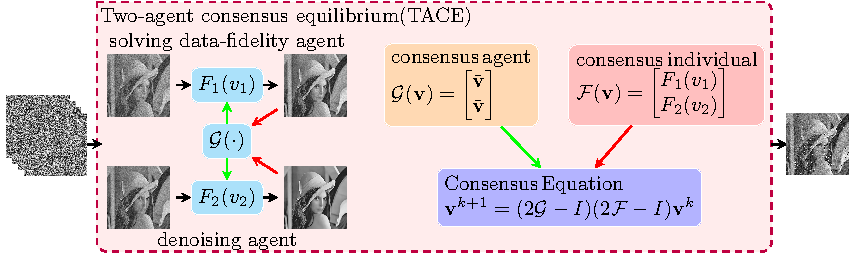
\includegraphics[width=\linewidth]{3-1}
	\caption{TACE算法示意图}\label{fig:3-1}
\end{figure}

\section{图像去噪算法的利普希茨约束}
当前流行的即插即用算法一般为非凸框架,虽然在图像反问题的求解上表现出色,但是算法的收敛性无法保证。为解决上述问题,Liu等人提出了实谱归一化(Real Spectral Normalization,realSN)方法以约束去噪器残差映射的利普希茨常数等于$1$,并给出了即插即用算法的收敛性保证\supercite{Ernest}。压缩映射与非扩张算子的定义如下所示:
\begin{definition} \label{def:3-1}
	算子$T:\mathbb{R}^n\to\mathbb{R}^n$是$L$-Lipschitz连续的,如果它满足
	\begin{equation}
		\Vert{T(x)-T(y)}\Vert_2^2\leq{L}\Vert{x-y}\Vert_2^2,\quad{\forall{x,y\in\mathbb{R}^n}}.
	\end{equation}
	若$L=1$,则$T$为非扩张算子;若$L<1$,则$T$为收缩算子。
\end{definition}

从泛函拟合的角度出发,DnCNN和IRCNN可用$D(y)=y-R(y)$表示,此时残差映射为$R(y)=y-D(y)=(I-D)(y)$。约束去噪器残差映射的利普希茨常数等价于迫使其满足如下假设:
\begin{assumption} \label{assumption:3-1}
	$\exists{\epsilon\ge{0}}$,$D_{\sigma}(x)\colon\mathbb{R}^n\to\mathbb{R}^n$对于$\forall{x,y}\in\mathbb{R}^n$满足:
	\begin{equation} 
		\Vert{(D_\sigma-I)(x)-(D_\sigma-I)(y)}\Vert^2\leq{\epsilon^2\Vert{x-y}\Vert^2}.
	\end{equation}	
\end{assumption}
%\begin{definition} \label{define:spectral-radius}
%	谱半径:$A_{n\times{n}}$的特征值为$\lambda_i$,$1\leq{i}\leq{n}$,那么其谱半径定义为
%	\begin{equation}
%		\rho(A) = \max_{1\leq{i}\leq{n}}\vert{\lambda_i}\vert.
%	\end{equation}
%\end{definition}
%\begin{definition} \label{define:spectral-norm}
%	谱范数:$A_{n\times{n}}$的谱范数定义为
%	\begin{equation}
%		\Vert{A}\Vert=\sup_{\Vert{x}\Vert=1}{\Vert{Ax}\Vert_2}.
%	\end{equation}
%\end{definition}
%bthm
%\begin{theorem} \label{third:com-spectral}
%	对于任意方阵$A_{n\times{n}}$,有
%	\begin{equation}
%		\Vert{A}\Vert=(\rho(A^{\mathit{H}}A))^{\frac{1}{2}}.
%	\end{equation}
%\end{theorem}
%\begin{lemma} \label{}
%	对于任意方阵$A_{n\times{n}}$,有
%	\begin{equation}
%		\Vert{A}\Vert\geq{\rho(A)}.
%	\end{equation}
%\end{lemma}
因DnCNN与IRCNN去噪器由卷积层、BN层、ReLU层复合而成,如图\ref{fig:2-7}和图\ref{fig:2-8}所示。此外ReLU函数的导数为1,故只需对卷积核$\mathcal{K}:\mathbb{R}^{C_{in}\times{h}\times{w}}\to{\mathbb{R}^{C_{out}\times{h}\times{w}}}$执行实谱归一化,其主要步骤如下所示:

(1)对卷积核应用一次幂迭代计算奇异值对应的特征向量:
\begin{equation} \label{equation:3-1}
	\begin{cases}
		V_{l}\leftarrow{\mathcal{K^\mathit{H}}(U_l)/\Vert{\mathcal{K^\mathit{H}}(U_l)}\Vert_2},\\
		U_{l}\leftarrow{\mathcal{K}(V_l)/\Vert{\mathcal{K}(V_l)}\Vert_2}.\\
	\end{cases}
\end{equation}

(2)计算卷积核的谱范数并进行归一化操作:
\begin{equation} \label{equation:3-2}
	\mathcal{K}_l\leftarrow{\mathcal{K}_l/\rho{(\mathcal{K_l})}}.
\end{equation}
其中$U_l\in\mathbb{R}^{C_{out}\times{h}\times{w}}$,$V_l\in\mathbb{R}^{C_{in}\times{h}\times{w}}$,$\rho(\mathcal{K}_l)=\left<{U_l, \mathcal{K}_l(V_l)}\right>$。以$\rho(\mathcal{K_l})/c_l$替代$\rho(\mathcal{K_l})$,此时深度学习去噪器利普希茨常数的上界为$C=\prod_{l=1}^L{c_l}$。关于去噪器有如下引理:
\begin{lemma} \label{lemma:3-1}
	若$D_{\sigma}:\mathbb{R}^n\to\mathbb{R}^n$满足假设\ref{assumption:3-1},当且仅当
	\begin{equation}
		\frac{1}{1+\epsilon}D_{\sigma}.
	\end{equation}
	为$\frac{\epsilon}{1+\epsilon}$-平均算子。更为一般地,$\frac{1}{1+2\epsilon}(2D_{\sigma}-I)$为$\frac{2\epsilon}{1+2\epsilon}$-平均算子。
\end{lemma}
当假设\ref{assumption:3-1}中的$\epsilon=1$时,由引理\ref{lemma:3-1}推的$\frac{1}{2}D_{\sigma}$为$\frac{1}{2}$-平均算子,亦为固定非扩张算子。

\section{基于即插即用先验的编码衍射成像算法}
对偶分解或ADMM等分解方法可以解决与图相关的问题,例如最大后验概率估计(Maximum Posteriori Estimation,MAP)推理和图匹配。其主要思想是将原始复杂图分解为更简单的子图,然后使用不同的机制重新组合这些子图。。大量图像重建任务可以表示为MAP问题\supercite{ZhangKai,Shunsuke,Stanley},其基本框架如下所示:
\begin{equation} \label{problem:3-1}
	\begin{aligned} 
		\hat{x}&=\arg\max_{x}\ p(x\;\vert\;y) \\
			   &=\arg\max_{x}\ -\log{p(y\;\vert\;x)-\log{p(x)}}.
	\end{aligned}
\end{equation}
其中条件概率${p(y\;\vert\;x)}$表示图像反问题的前向模型,$p(x)$表示待恢复图像的先验分布。MAP为基于模型的图像重建方法,其关键在于寻找待恢复图像的有效先验知识。根据帕累托法则,待恢复图像的先验知识起关键性作用。另外,MAP等价于求解如下优化问题:
\begin{equation} \label{problem:3-2}
	\mathop{\text{minimize}}\limits_{x}\quad f(x)+\lambda{g(x)}.
\end{equation}
其中$f(x)\overset{\underset{\mathrm{def}}{}}{=}{-\log{p(y\vert{x})}}$为${p(y\;\vert\;x)}$的负最大似然估计函数,$g(x)\overset{\underset{\mathrm{def}}{}}{=}{-\log{p(x)}}$。问题\eqref{problem:3-2}为标准的无约束优化问题。站在贝叶斯优化的视角,编码衍射成像模型的数据保真项应正比于其条件概率对应的负最大似然函数。一般地,编码衍射成像的观测模型为$y=\vert{Ax}\vert+w$,其中$w\sim{C\mathcal{N}(0,\sigma_w{I})}$,则负的最大似然函数$-\log{p(y\vert{x})}\propto\frac{1}{2}{\Vert{y-\vert{Ax}\vert}\Vert_2^2}$。此时求解编码衍射中的PR问题,只需令$f(x)=\frac{1}{2}{\Vert{y-\vert{Ax}\vert}\Vert_2^2}$即可。另外,图像的先验知识$\log{p(x)}$对非线性图像反问题求解至关重要。人们根据图像的先验分布提出了大量有效的图像去噪算法:基于稀疏表示的K-SVD去噪方法利用图像块的自适应字典学习有效地去除噪声;BM3D综合稀疏性和局部自相似性取得了传统算法中SOTA的结果。

相反地,深度学习技术利用大量数据学习图像先验,基于监督学习的DnCNN和IRCNN从海量的训练数据中学习到的先验知识具有更强的泛化能力和更复杂的参数化表达,且无需调节算法参数以适应不同的应用场景\supercite{Kai,ZhangKai};基于无监督学习的深度图像先验方法利用生成器网络的结构足以在任何学习之前捕获大量的低级图像统计信息进行去噪处理;传统的去噪算法的深度展开(Deep Unrolling)策略也在图像去噪领域取得了一定的进展\supercite{Yan,Chenyang,Hasselt,Schaul,Bellemare,Matteo,Dabney1,Dabney2,Volodymyr}。一般地,图像先验$\log{p(x)}$有明确的数学表达式,这表明优化问题\ref{problem:3-2}是显式地,仍属于优化领域的范畴。但是当图像先验$\log{p(x)}$不能转化为数学表达式,优化问题\eqref{problem:3-2}为隐式地,脱离了优化领域的范畴。如何利用去噪器构造图像或隐式地嵌入到结构化求解算法中需要进一步研究。即插即用ADMM算法是一种强大的图像重建框架,允许高级图像去噪先验集成到物理系统前向模型中生成高质量的图像重构结果。Venkatakrishnan等人首次提出即插即用先验的概念,根据ADMM框架的特殊结构,提出了即插即用先验(Plug-and-Play Priors, $P^3$)算法\supercite{Stanley}。该算法在求解正则化的图像反问题时,将ADMM框架分成数据保真项模型和去噪模型(先验模型),数据保真项模型通过简单的梯度下降法或存在快速求解算法(去模糊中的模糊核为循环矩阵,可用快速傅里叶变换求解),去噪模型利用传统的去噪算法或基于深度学习的去噪算子进行求解。 

由于去噪模型可利用不同的去噪算子进行求解,$P^3$算法能够利用不同的图像先验进行图像重建。Chan等人假设去噪器有界:$\Vert{D_{\sigma}(x)-x}\Vert/n\leq{\sigma^2C}$,而有界去噪器是渐近不变地:$D_{\sigma}\to{0}(\sigma\to{0})$。之后,Chan等人从理论上在$f(x)$的$\mu$-强凸的假设下,证明了即插即用ADMM算法的不动点收敛性\supercite{ZhangKai}。Metzler等人将BM3D去噪算子引入到近似消息传递算法的迭代中,隐式地利用即插即用先验求解压缩相位恢复问题,并且在去噪器满足假设:$\mathbb{E}\left[\Vert{D_{\sigma}(x+\sigma\epsilon)-x}\Vert^2/n\right]\leq{\kappa\sigma^2}$和观测矩阵$\{a_j\overset{\underset{\mathrm{iid}}{}}{\sim}\mathcal{N}(0,I_n)\}_{1\leq {j\leq{m}}}$下,证明了prGAMP算法的收敛性\supercite{Metzler4}。数值实验结果表明prGAMP算法能够从欠采样测量数据中重建高质量图像。

基于隐式先验的图像重建算法具有有效、灵活的特点,该类算法能够利用高级去噪器将图像的先验知识隐式地引入到图像重建中。但是即插即用ADMM算法严重依赖于ADMM算法的结构,并且为非凸框架,收敛性与收敛速度无法保证。为了有效解决该问题,Liu等人提出实谱归一化技术对深度去噪器DnCNN进行利普希茨约束\supercite{Ernest}。令人诟病的是该方法仅限于深度学习去噪器,并未涉及图像反问题中的数据保真项,使得基于即插即用先验的ADMM算法应用范围有限。

鉴于此,Romano等人提出了显式的RED先验,与隐式即插即用先验的不同之处在于其具有明确的数学表达式,因而优化问题\eqref{problem:3-2}明确。此外,Siavash等人构造了另一种显式的自编码先验$\frac{1}{2}\Vert{x-D_{\sigma}(x)}\Vert_2^2$\supercite{Siavash,Yankun,Zhang}。另外,基于即插即用先验的的PR算法能够依据最大似然估计设计针对不同测量系统噪声类型的数据保真项,但Metzler发现泊松噪声可以应用数据保真项$\frac{1}{2}{\Vert{y-\vert{Ax}\vert}\Vert_2^2}$进行求解,打破了依据最大似然估计设计数据保真项的限制。以下介绍两种基于近邻算子的即插即用算法。

\subsection{即插即用ADMM算法}
即插即用算法是将ADMM或其他邻近算法与高级去噪器先验相结合的非凸框架。PR问题中代价函数$f(x)=\frac{1}{2}{\Vert{y-\vert{Ax}\vert}\Vert_2^2}$非凸、非光滑。利用ADMM方法求解优化问题\eqref{problem:3-2},该问题等价于
\begin{equation} \label{problem:3-3}
	\begin{aligned} 
		&\text{minimize}\quad\frac{1}{2}{\Vert{y-\vert{Az}\vert}\Vert_2^2}+\lambda{g(x)} \\
		&\text{subject\ to}\quad x-z=0 \\
	\end{aligned}
\end{equation}
上述优化问题转化为以下增广拉格朗日函数为:
\begin{equation} \label{equation:3-3}
	\begin{aligned}
		L_{\rho}(x,y,z)&=\frac{1}{2}{\Vert{y-\vert{Az}\vert}\Vert_2^2}+\lambda{g(x)}+y^\top(x-z)+\frac{\rho}{2}\Vert{x-z}\Vert_2^2\\
		&=\frac{1}{2}{\Vert{y-\vert{Az}\vert}\Vert_2^2}+\lambda{g(x)}+\frac{\rho}{2}\Vert{x-z+u}\Vert_2^2.
	\end{aligned}
\end{equation}
其中$u=\frac{y}{\rho}$表示尺度对偶变量,ADMM方法通过求解以下子问题(对于第$k+1$次迭代)对上述优化问题进行求解:

(1)图像$x$去噪子问题:固定$z,u$,问题\eqref{equation:3-3}相当于求解以下子问题:
\begin{equation} \label{}
	x^{k+1}=\arg\min_{x}=\lambda{g(x)}+\frac{\rho}{2}\Vert{x-z^k+u^k}\Vert_2^2.
\end{equation}
上述子问题与基于先验的去噪问题相似,故数值解为:
\begin{equation} \label{third:x-step}
	x^{k+1}:=D_{\sigma}(z^k-u^k).
\end{equation}

(2)辅助变量$z$更新子问题:固定$x,u$,问题\eqref{equation:3-3}相当于求解以下子问题:
\begin{equation} \label{equation:3-4}
	z^{k+1}=\arg\min_{z}=\frac{1}{2}{\Vert{y-\vert{Az}\vert}\Vert_2^2}+\frac{\rho}{2}\Vert{x^{k+1}-z+u^k}\Vert_2^2.
\end{equation}
应用不动点迭代,上述问题的数值解为:
\begin{equation} \label{equation:3-5}
	z^{k+1}:=\frac{1}{1+\rho}\left({A^{\mathit{H}}\left(\frac{Az^k}{\vert{Az^k}\vert}\odot{y}\right)}+\rho{(x^{k+1}+u^k)}\right).
\end{equation}

(3)对偶变量$u$更新:
\begin{equation} \label{equation:3-6}
	u^{k+1}:=u^k+x^{k+1}-z^{k+1}.
\end{equation}

(4)最后应用内插技术得到:
\begin{equation} \label{equation:3-7}
	\hat{x}^{k+1} := (1-\alpha)\hat{x}^k+\alpha{x^k}.
\end{equation}
算法的终止条件利用优化变量的相对残差范数(relative residual, res)进行度量,其定义为:
\begin{equation} \label{equation:3-8}
	\text{res}=\frac{\Vert{x^{k+1}-x^k}\Vert_2}{\max\{1, \Vert{x^k}\Vert_2\}}.
\end{equation}
当$\text{res}\leq{\epsilon}$($\epsilon$为相对误差限)或达到最大迭代次数算法终止迭代。算法\ref{algorithm:3-1}总结了即插即用ADMM算法。
\begin{algorithm}[!htbp]
	\setstretch{1.4}\zihao{-4}
	\caption{即插即用ADMM(PnP-ADMM)}
	\label{algorithm:3-1}
	\begin{algorithmic}[1]
		\REQUIRE	观测值$y\in \mathbb{R}^m$; % this command shows "Input"
		\ENSURE		% this command shows "Initialized"
		$\rho > 0, \alpha\in (0,1), \sigma\in[1,50], (x^0,z^0,u^0)$随机; \\
		\WHILE {\emph{not converged}}
		\STATE	$x^{k+1}:=(1-\alpha)x^k + \alpha{D_{\sigma}(z^k-u^k)}$; \\ % line number at left side
		\STATE	$z^{k+1}:=\frac{1}{1+\rho}\left({A^{\mathit{H}}\left(\frac{Az^k}{\vert{Az^k}\vert}\odot{y}\right)}+\rho{(x^{k+1}+u^k)}\right)$; \\	% line number at left side
		\STATE	$u^{k+1}:=u^k+x^{k+1}-z^{k+1}$; \\ % line number at left side
		\ENDWHILE
		\RETURN 重构图像$x^{k+1}$. % this command shows "Output"
	\end{algorithmic}
\end{algorithm}

\subsection{即插即用邻近梯度算法}
利用邻近梯度方法求解优化问题\eqref{problem:3-2},第$k+1$次迭代的公式如下所示:
\begin{equation} \label{equation:3-9}
	x^{k+1}:=D_{\sigma}\left(x^k-\eta_k{A^{\mathit{H}}\left({Ax^k-y\odot{\frac{Ax^k}{\vert{Ax^k}\vert}}}\right)}\right).
\end{equation}
加速近邻梯度法在外推处求代价函数的梯度,可看作是Nerterov's加速算法的推广。其对应的第$k+1$次迭代的公式如下所示:
\begin{equation} \label{equation:3-10}
	\begin{cases}
		v^{k+1}:=x^k+\omega_k(x^k-x^{k-1}), \\
		x^{k+1} := D_{\sigma}\left(v^k-\eta_k{A^{\mathit{H}}\left({Av^k-y\odot{\frac{Av^k}{\vert{Av^k}\vert}}}\right)}\right). \\
	\end{cases}
\end{equation}
其中$\eta_k\in(0,\frac{1}{L})$,$L$为数据保真项梯度的利普希茨常数,而数据保真项非光滑,故数据保真项的梯度不满足利普希茨连续性条件。$\omega_k$的典型值为$\frac{k}{k+3}$。上述算法的迭代终止条件与算法\ref{algorithm:3-1}相同。算法\ref{algorithm:3-2}总结了即插即用邻近梯度算法。
\begin{algorithm}[!htbp]
	\setstretch{1.4}\zihao{-4}
	\caption{即插即用FBS(PnP-FBS)}
	\label{algorithm:3-2}
	\begin{algorithmic}[1]
		\REQUIRE	观测值$y\in \mathbb{R}^m$;	% this command shows "Input"
		\ENSURE		% this command shows "Initialized"
		$\eta_k\in(0,\frac{1}{L}),\sigma\in[1,50],x^0$随机; \\
		\WHILE {\emph{not converged}}
		\STATE $x^{k+1}:=D_{\sigma}\left(x^k-\eta_k{A^{\mathit{H}}\left({Ax^k-y\odot{\frac{Ax^k}{\vert{Ax^k}\vert}}}\right)}\right)$;\\ % line number at left side
		\ENDWHILE
		\RETURN 重构图像$x^{k+1}$. % this command shows "Output"
	\end{algorithmic}
\end{algorithm}

\section{基于去噪正则化先验的编码衍射成像算法}
RED(Regularization by Denoising)最早由Romano等人提出\supercite{Romano,Hong,Zihui},用于解决图像去模糊、单幅图像超分辨率、相位恢复等图像反问题。RED正则项的数学表达式为:
\begin{equation} \label{equation:3-11}
	g(x)=\frac{1}{2}x^\top(x-D_{\sigma}(x)).
\end{equation}
若式\eqref{equation:3-11}满足:

(1)局部齐次性(local homogeneity):$D_{\sigma}(Cx)=CD_{\sigma}(x),\vert{C-1}\vert\leq\epsilon$;

(2)其梯度谱半径小于等于$1$:$\rho(\nabla_{x}D_{\sigma}(x))\leq{1}$;

由(1)(2)可推的$g(x)$为凸函数,并且$\nabla{g(x)}=x-D_{\sigma}(x)$。因为$\rho(\nabla_{x}D_{\sigma})\leq\Vert{D_{\sigma}}\Vert_2$,所以实谱归一化的DnCNN和IRCNN满足条件(2)。图\ref{fig:3-1}为$D_{\sigma}((1+\epsilon)x)$相对于$(1+\epsilon)D_{\sigma}(x)$的散点图,括号中的数字表示两者的方差,实验图像$x$为Lenna,$\sigma=15$。可见DnCNN、IRCNN、Realsn-DnCNN和Realsn-IRCNN均满足条件(1)。
\begin{figure}[!htbp]
	\vspace*{-0.05\linewidth}
	\centering
	\subfigure[DnCNN(3.74e-4)]{
		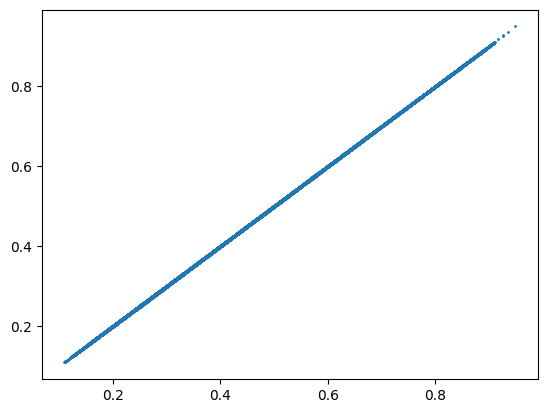
\includegraphics[width=0.4\linewidth]{3-2-1}  
	}
	\subfigure[IRCNN(3.33e-4)]{
		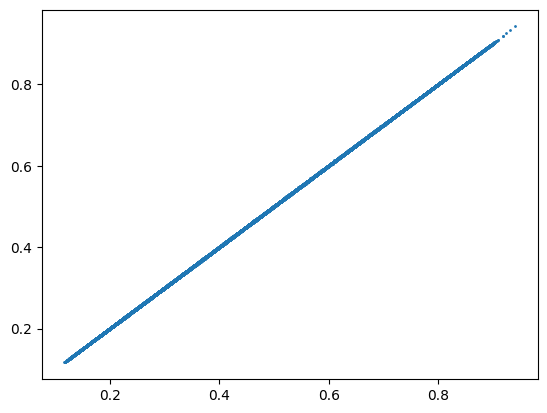
\includegraphics[width=0.4\linewidth]{3-2-2}  
	}
	
	\subfigure[realSN-DnCNN(3.49e-4)]{
		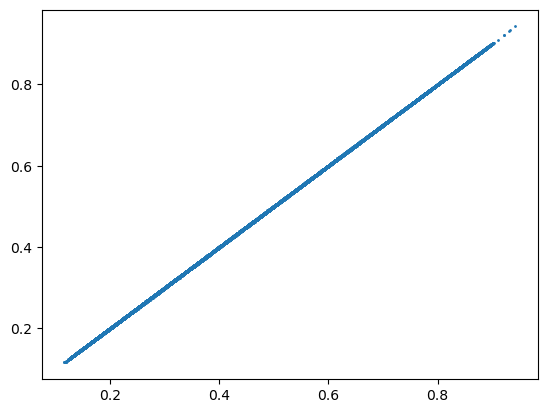
\includegraphics[width=0.4\linewidth]{3-2-3}  
	}
	\subfigure[realSN-IRCNN(3.47e-4)]{
		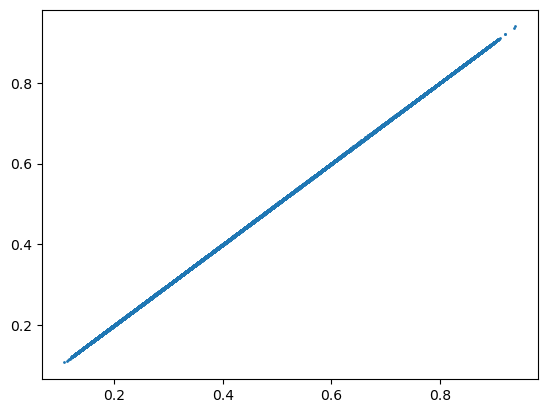
\includegraphics[width=0.4\linewidth]{3-2-4}  
	}
	\caption{去噪器DnCNN与IRCNN的局部齐次性评估散点图} \label{fig:3-2}
\end{figure}

RED正则项可看作是图像$x$与相应残差$x-D_{\sigma}(x)$的非归一化自相关性,当残差趋于零值时,图像$x$应满足$x\approx{D_{\sigma}(x)}$;当图像$x$与其残差图像$x-D_{\sigma}(x)$不相关时,$g(x)$趋向于零值。Metzler等人将RED作为相位恢复的正则项,提出了基于RED先验的prDeep算法\supercite{Metzler1}。prDeep算法用于恢复含泊松噪声的观测值,但其对应的PR问题如下所示:
\begin{equation} \label{problem:3-4}
	\mathop{\text{minimize}}\limits_{x}\quad \frac{1}{2}{\Vert{y-\vert{Ax}\vert}\Vert_2^2} + \frac{\lambda}{2}x^\top(x-D_{\sigma}(x)).
\end{equation}
RED先验对应的proximal算子为:
\begin{equation} \label{equation:3-12}
	\begin{aligned} 
		\text{prox}_{g}(v)&=\arg\min_{x}\frac{\lambda}{2}x^\top(x-D_{\sigma}(x))+\frac{1}{2}\Vert{x-v}\Vert_2^2,\\
		&=u_{\infty},
	\end{aligned}
\end{equation}
其中$u_j=\frac{1}{1+\lambda}(u_{j-1}+\lambda{D_{\sigma}(u_{j-1})})$,$u_0=v$。由于去噪器迭代存在大量计算,故一般取$j=1$。Metzler利用FASTA算法进行求解,与PnP-FBS算法基本相同,但FASTA采取自适应学习率和反向线性搜索技术进行加速,使得重建速度优于PnP-FBS\supercite{Goldstein}。有趣的是,PrDeep作者在实验中选取噪声强度固定的去噪算子,但本章发现选取$\sigma\in[1,50]$的盲去噪器仍可以取得与之相当的重构效果。

\section{从共识优化到共识方程}
图像重构中正则化反问题的方法由于其能够结合复杂的物理传感器模型和有效的正则化特点而得到广泛应用\supercite{Gregery,Joon,Kamilov,Siavash,Yankun,Zhang}。基于即插即用先验的方法提供了一个使用高级去噪算法作为正则化器的框架。然而,将正则化的反问题作为优化问题的解决方案,限制了可能的正则化条件和物理传感器模型的多样性。

在一般的动力系统中,存在多个传感器收集多组数据的情况。其对应的代价函数被分解为多个辅助函数之和的形式:
\begin{equation} \label{problem:3-5}
	\mathop{\text{minimize}}\limits_{x}\quad f(x)=\sum_{i=1}^{N}\mu_{i}f_i(x),
\end{equation} 
其中$x\in\mathbb{R}^n$,$f_i\colon\mathbb{R}^n\to\mathbb{R}\cup\{+\infty\}$,权重$\mu_{i}>0$,$i=1,\ldots,N$并且$\sum_{i=1}^{N}{u_i}=1$。在共识优化中,最小化原始代价函数可重新表述为辅助函数之和的最小化,约束中每个分离的优化变量$x_i$共享同一个$x$:
\begin{equation} \label{problem:3-6}
	\begin{aligned}
		&\text{minimize}\quad\sum_{i=1}^{N}\mu_{i}f_i(x) \\
		&\text{subject\ to}\quad{x_{i} = x,\ i=1,\ldots,N} \\
	\end{aligned}
\end{equation}
其中$x\in\mathbb{R}^n$,$x_{i}\in\mathbb{R}^n$。上述优化问题可用ADMM算法进行求解。正则化的反问题和优化问题得益于广泛的理论和强大的算法,但是,大量有效、简单的去噪算法不能嵌入到优化算法中。即使优化算法(例如ADMM)的结构性允许嵌入,但该算法一般为隐式模型,无法保证去噪迭代对应近邻算子的存在,导致代价函数无法显示地确定。再者,该算法为非凸算法,收敛性无法保证。不过该算法一般收敛到不动点,它对去噪迭代通过迭代控制前向模型的近邻算子中的步长和去噪器的噪声强度鲁棒。以下将从共识优化推到共识方程:

假设$f_i\colon\mathbb{R}^n\to\mathbb{R}\cup\{+\infty\}$为闭凸函数,$F_i$为相应的近邻算子,其由式\eqref{proximal-operator}定义。优化问题\eqref{problem:3-6}对应的拉格朗日函数为
\begin{equation} \label{equation:3-13}
	L(x,(x_i)_{i=1}^N,(\lambda_i)_{i=1}^N)=\sum_{i=1}^{N}(\gamma\mu_{i}f_i(x_i)+\lambda_i^\top(x-x_i)).
\end{equation}
其中$\gamma$为近邻算子$F_i$的尺度因子,$\lambda_i$为朗格朗日乘子向量。如果$f_i$是凸函数和下半连续的,则KKT条件是最优解的充分条件。最优解$(x^*,(x_i^*)_{i=1}^N,(\lambda_i^*)_{i=1}^N)$由式\eqref{equation:3-14}给出:
\begin{equation} \label{equation:3-14}
	\begin{aligned}
 		\nabla_x{L(x^*,(x_i^*)_{i=1}^N,(\lambda_i^*)_{i=1}^N)}&=0, \\
		\partial_{x_i}{L(x^*,(x_i^*)_{i=1}^N,(\lambda_i^*)_{i=1}^N)}&\ni{0},\quad\forall{i=1,\ldots,N}, \\
		x_i^*-x^*&=0,\quad\forall{i=1,\ldots,N}. \\
	\end{aligned}
\end{equation}
其中$\partial_{x_i}$表示子微分。式\eqref{equation:3-14}转化为:
\begin{equation} \label{equation:3-15}
	\begin{aligned}
		\sum_{i=1}^{N}\lambda_i&=0, \\
		\gamma\mu_i\partial{f_i(x_i^*)}&\ni{\lambda_i^*},\quad\forall{i=1,\ldots,N}, \\
		x_i^*&=x^*,\quad\forall{i=1,\ldots,N}. \\
	\end{aligned}
\end{equation}
定义$u_i^*=\lambda_i^*/\mu_i$,将$x_i^*=x^*$代入$\gamma\mu_i\partial{f_i(x_i^*)}\ni{\lambda_i^*}$得到$\gamma\partial{f_i(x^*)}\ni{u_i^*}$。再两边同时加$x^*$得到$x^*+\gamma\partial{f_i(x^*)}\ni{x^*+u_i^*}$。此式等价于
\begin{equation} \label{equation:3-16}
	(I+\gamma\partial{f_i})(x^*)\ni{x^*+u_i^*}.
\end{equation}
由式\eqref{equation:3-16}推的$x^*=(I+\gamma\partial{f_i})^{-1}(x^*+u_i^*)$,此式正是$f_i$的近邻算子$F_i$。由以上可得共识方程为
\begin{equation} \label{equation:ce}
	\begin{aligned}
		F_i(x^*+u_i^*)&=x^*,\quad{i=1,\ldots,N,} \\
		\overline{\mathbf{u}}_\mu^*&=0. \\
	\end{aligned}
\end{equation}
其中$\mathbf{u}\in\mathbb{R}^{nN}$为$u_1,\ldots,u_N$的列向堆叠,$\overline{\mathbf{u}}_\mu$为权重平均$\sum_{i=1}^{N}\mu_i{u_i}$。

\section{基于共识方程的编码衍射成像算法}
共识均衡(Consensus Equilibrium)旨在利用迭代求解算法使得不同算子达到平衡点,类似于博弈论中的纳什均衡(Nash Equilibrium)。共识方程\eqref{equation:ce}脱离了优化算法的范畴,求解目标有着清晰的数学表示,是一个优雅的数学框架。共识方程可将基于优化的算子(近邻算子)或基于非优化的算子(去噪器)嵌入其中,每一个算子代表一个博弈主体,允许多个主体参与非合作式博弈。

Chan等人将CE用于图像盲去噪与非理想背景中前景自动提取\cite{Gregery,Xiran},在噪声未知的情况下取得了SOTA结果\supercite{Gregery,Joon,Xiran}。但对于确定的噪声强度的噪声,去噪性能不如单个DnCNN。基于多代理CE的前景自动提取算法融合TV去噪、背景提取、 Alpha matting等代理,以处理背景不完美的复杂场景。受到Chan等人工作的启发,本节将CE用于编码衍射模型中的相位恢复问题,提出了TACE(Two-agent Consensus Equilibrium)算法,以下为主要求解步骤。

CE方程为无约束的方程组,可用非扩张算子的不动点理论去分析其收敛性。另外,非扩张算子的预处理各向异Mann迭代可用于算法的加速处理。首先,定义如下概念:
\begin{equation} \label{equation:agent}
	\mathbf{F}(\mathbf{v})
	=
	\begin{pmatrix}
		F_1(v_1) \\ F_2(v_2)
	\end{pmatrix} 
	=	
	\begin{pmatrix}
		((1-\theta)I+\theta\text{prox}_{\gamma{f}})(v_1) \\ \frac{1}{2}D_{\sigma}(v_2)
	\end{pmatrix} 
	\quad and \quad
	\mathbf{G}_{\mu}(\mathbf{v})
	=
	\begin{pmatrix}
		\overline{\mathbf{v}}_{\mu} \\ \overline{\mathbf{v}}_{\mu} 
	\end{pmatrix} 
\end{equation}
其中
\begin{equation} \label{equation:3-17}
	\begin{aligned}
		\text{prox}_\gamma{f}(v_1)&=\arg\min_{x}
		\frac{1}{2}{\Vert{y-\vert{Ax}\vert}\Vert_2^2} +\frac{1}{2\gamma}{\Vert{x-v_1}\Vert_2^2}, \\
		&\approx\frac{1}{1+\gamma}\left({\gamma A^{\mathit{H}}\left(\frac{Ax^k}{\vert{Ax^k}\vert}\odot{y}\right)}+v_1^k\right),\; k\geq{0}.
	\end{aligned}
\end{equation}
如果$\mathbf{v}^*=\hat{x}^*+\mathbf{u}^*$,其中$\hat{x}=(x,x)^\top$,满足$\overline{\mathbf{v}}_{\mu}^*=x^*$,并且
\begin{equation} \label{equation:3-18}
	\left({2\mathbf{G}_{\mu}-I}\right)\left({2\mathbf{F}-I}\right)\mathbf{v}^*=\mathbf{v}^*.  
\end{equation}
则$(x^*,\mathbf{u}^*)$为CE方程\ref{equation:ce}当$N=2$时的最优解。定义$\mathbf{T}\overset{\underset{\mathrm{def}}{}}{=}\left({2\mathbf{G}_{\mu}-I}\right)\left({2\mathbf{F}-I}\right)$,应用非扩张算子的Mann迭代可得CE方程的第$k$次迭代为:
\begin{equation} \label{equation:3-19}
	\begin{aligned}
		\mathbf{v}^{k+1}&:=(1-\beta)\mathbf{v}^{k}+\beta\mathbf{T}(\mathbf{v}^{k}),	\\
		x^{k+1}&:=\overline{\mathbf{v}}^{k+1}.
	\end{aligned}
\end{equation}
最后再对优化变量$x$应用内插技术得到以下算法:
\begin{equation} \label{equation:3-20}
	\begin{aligned}
		\mathbf{v}^{k+1}&:=(1-\beta)\mathbf{v}^{k}+\beta\mathbf{T}(\mathbf{v}^{k}),	\\
		x^{k+1}&:=(1-\alpha)x^k + \alpha\overline{\mathbf{v}}^{k+1}.
	\end{aligned}
\end{equation}
算法\ref{algorithm:3-3}总结TACE算法的实现细节。
\begin{algorithm}[!htbp]
	\setstretch{1.4}\zihao{-4}
	\caption{TACE}
	\label{algorithm:3-3}
	\begin{algorithmic}[1]
		\REQUIRE	观测值$y\in \mathbb{R}^m$; % this command shows "Input"
		\ENSURE		% this command shows "Initialized"
		$\alpha,\beta\in (0,1), \theta\in(0,\frac{1}{2}],\gamma{=1}, sigma\in[1,50], \mu_{1}=\mu_{2}=\frac{1}{2},(\mathbf{v}^0,x^0)$随机; \\
		\WHILE {\emph{not converged}}
		\STATE	$\mathbf{v}^{k+1}:=(1-\beta)\mathbf{v}^{k}+\beta\mathbf{T}(\mathbf{v}^{k})$; \\  % line number at left side
		\STATE	$x^{k+1}:=(1-\alpha)x^k + \alpha\overline{\mathbf{v}}_{\mu}^{k+1}$; \\	% line number at left side
		\ENDWHILE
		\RETURN 重构图像$x^{k+1}$.  % this command shows "Output"
	\end{algorithmic}
\end{algorithm}
需要指出的是,当$N=2$时,PnP-ADMM和TACE的最优解等价,均收敛到不动点$(x^*, u^*)$,即满足式\eqref{equation:3-21}:
\begin{equation} \label{equation:3-21}
	\begin{aligned}
		\text{prox}_{\gamma{f}}(x^*-u^*)&=x^*, \\
		D_{\sigma}(x^*+u^*)&=x^*. \\
	\end{aligned}
\end{equation}
不失一般性,TACE算法的推广版本MACE(Multi-Agent Consensus
Equilibrium)算法的第$k+1$次迭代如图\ref{fig:3-3}所示。图\ref{fig:3-3}中$F_{1},\ldots,F_{N}$表示$N$个代理。
\begin{figure}[!hptb]
	\centering
	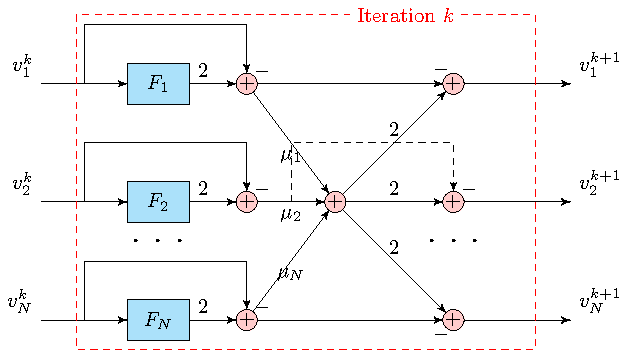
\includegraphics[width=0.8\linewidth]{3-3}
	\caption{MACE算法第$k+1$次迭代示意图}\label{fig:3-3}
\end{figure}

最后,在理论层面当$F^\prime{s}$满足假设\ref{assumption:3-2}时,本章通过严格的数学证明给出了MACE算法的收敛性,此时文献\cite{Xiran}的假设条件可看作是下述结论当$\theta=\frac{1}{2}$时的一个特例。收敛性结论如下所示:
\begin{assumption} \label{assumption:3-2}
	$\exists{\theta\in(0,\frac{1}{2}]}$,$F_{i}\colon\mathbb{R}^{n}\to\mathbb{R}^{n}$满足
	\begin{equation}
		F_i=(1-\theta)I+\theta{R_i},\quad{i=1,\ldots,N},
	\end{equation}
	其中$R_i$为非扩张算子。
\end{assumption}
\begin{lemma}\label{lemma:3-2}
	假设$f$为闭凸函数(Convex Closed Proper,CCP),则其微分算子$\partial{f(x)}$的预解算子(Resolvent Operator)$R=(I+\gamma{\partial{f(x)}})^{-1}$固定非扩张,从而Cayley算子$C=2R-I=2(I+\gamma{\partial{f(x)}})^{-1}-I$非扩张。
\end{lemma}
\begin{proof}
	由于$f$为凸函数,可以得到$(\partial{f(x)}-\partial{f(y)})^\top(x-y)\geq{0}$,
	再令$(x,u),(y,v)\in{R}$,那么有$x\in{u+\gamma\partial{f(u)}}$,$y\in{v+\gamma\partial{f(v)}}$。
	上述两式相减,可得
	\begin{equation} \label{equation:3-24}
		x-y\in{u - v + \gamma(\partial{f(u)}-\partial{f(v)})}.
	\end{equation}
	使用$(u-v)^\top$左乘式\eqref{equation:3-24}并综合$(\partial{f(x)}-\partial{f(x)})\top{x-y}\geq{0}$,可得
	\begin{equation}
		\Vert{u-v}\Vert_2^2\leq(u-v)^\top(x-y).
	\end{equation}
	因此就有
	\begin{equation}
		\begin{aligned}
			\Vert{C(x)-C(y)}\Vert_2^2
			&=4\Vert{u-v}\Vert_2^2-4(u-v)^\top(x-y)+\Vert{x-y}\Vert_2^2 \\
			&\leq{\Vert{x-y}\Vert_2^2}.
		\end{aligned}
	\end{equation}
	令$R=\frac{1}{2}I+\frac{1}{2}(2R-I)$,可得算子$R$固定非扩张。
\end{proof}
\begin{lemma}\label{lemma:3-3}
	若$\tau\in(0,\frac{1}{2})$,$S\colon\mathbb{R}^n\to\mathbb{R}^n$为$\tau$-平均算子则$2S-I$为$2\tau$-平均算子。
\end{lemma}
\begin{proposition}
	令$\mathbf{F}$与$\mathbf{G}_{\mu}$定义为式\eqref{equation:agent},且$\mathbf{T}=\left({2\mathbf{G}_{\mu}-I}\right)\left({2\mathbf{F}-I}\right)$。若$\mathbf{F}$满足假设\ref{assumption:3-2}则$T$为非扩张算子。
\end{proposition}
\begin{proof}令$\mathbf{x}$,$\mathbf{y}\in\mathbb{R}^{nN}$。
	情形--$1$($\theta=\frac{1}{2}$):当$\theta=\frac{1}{2}$时,$F^\prime{s}$均为固定非扩张算子($\frac{1}{2}$-平均算子),那么
	\begin{equation}
		\begin{aligned}
			\Vert{\mathbf{F}(\mathbf{x})-\mathbf{F}(\mathbf{y})}\Vert_2^2
			&=\sum_{i=1}^{N}\left(F_i(x_i)-F_i(y_i)\right)^2 \\
			&\leq\left\langle{\mathbf{x}-\mathbf{y},\mathbf{F}(\mathbf{x})-\mathbf{F}(\mathbf{y})}\right\rangle.
		\end{aligned} 
	\end{equation}
	因此
	\begin{equation}
		\begin{aligned}
			\Vert{(2\mathbf{F}-\mathbf{I})(\mathbf{x})-(2\mathbf{F}-\mathbf{I})(\mathbf{y})}\Vert_2^2 &=4\Vert{\mathbf{F}(\mathbf{x})-\mathbf{F}(\mathbf{y})}\Vert_2^2-4\left\langle{\mathbf{x}-\mathbf{y},\mathbf{F}(\mathbf{x})-\mathbf{F}(\mathbf{y})}\right\rangle+\Vert{\mathbf{x}-\mathbf{y}}\Vert_2^2\\
			&\leq\Vert{\mathbf{x}-\mathbf{y}}\Vert_2^2.
		\end{aligned} 
	\end{equation}
	显然$\mathbf{G}_{\mu}^\top=\mathbf{G}_{\mu}$,从而可以有$(2\mathbf{G}_{\mu}-\mathbf{I})^\top=2\mathbf{G}_{\mu}-\mathbf{I}$,即$\Vert{(2\mathbf{G}_{\mu}-\mathbf{I})\mathbf{x}}\Vert_2^2=\Vert{x}\Vert_2^2$。
	所以
	\begin{equation}
		\begin{aligned}
			\Vert{(2\mathbf{G}_{\mu}-\mathbf{I})[(2\mathbf{F}-\mathbf{I})(\mathbf{x})]-(2\mathbf{G}_{\mu}-\mathbf{I})[(2\mathbf{F}-\mathbf{I})(\mathbf{y})]}\Vert_2^2 
			&=\Vert{(2\mathbf{F}-\mathbf{I})(\mathbf{x})-(2\mathbf{F}-\mathbf{I})(\mathbf{y})}\Vert_2^2\\
			&\leq\Vert{\mathbf{x}-\mathbf{y}}\Vert_2^2.
		\end{aligned}
	\end{equation}
	
	情形--$2$($\theta\in(0,\frac{1}{2})$):当$\theta\in(0,\frac{1}{2})$时,$F^\prime{s}$均为$\theta$-平均算子,那么
	\begin{equation} \label{equation:3-25}
		\begin{aligned}
			\Vert{\mathbf{F}(\mathbf{x})-\mathbf{F}(\mathbf{y})}\Vert_2^2+(1-2\theta)\Vert{\mathbf{x}-\mathbf{y}}\Vert_2^2\leq{2(1-\theta)}\left\langle{\mathbf{x}-\mathbf{y},\mathbf{F}(\mathbf{x})-\mathbf{F}(\mathbf{y})}\right\rangle .
		\end{aligned} 
	\end{equation}
	式\eqref{equation:3-25}结合引理\ref{lemma:3-3}可得$2\mathbf{F}-\mathbf{I}$为$2\theta$-平均算子,所以$\mathbf{T}$为$\frac{1}{2(1-\theta)}$-平均算子,从而$T$为非扩张算子。
\end{proof}

\section{实验结果及分析}
本章的实验分为三部分:(1)实谱归一化深度图像去噪算子DnCNN与IRCNN的有效性验证;(2)TACE算法抗高斯噪声对比实验;(3)TACE算法抗泊松噪声对比实验。本节算法的实验仿真平台为Intel(R) Xeon(R) CPU E5-2650 v4处理器(2.20GHz),252G内存,ubuntu 16.04操作系统, Tesla K80显卡,cuda 10.2,cudnn 7605。

\subsection{实谱归一化有效性验证}
训练数据与测试数据:本节使用上述图像去噪算法来进行噪声去除。训练数据为BSD400,测试数据为Set12。DnCNN和IRCNN的网络结构与超参数与原文保持一致\supercite{Kai}。对比的算法包括BM3D、非盲DnCNN(DnCNN-S)、盲DnCNN(DnCNN-B,$\sigma=1\sim{50}$)、非盲IRCNN(IRCNN-S)、盲IRCNN(IRCNN-B,$\sigma=1\sim{50}$)和实谱归一化的版本(realSN)。表\ref{table:3-1}和表\ref{table:3-2}给出了不同算法的PSNR对比结果。
\begin{table}[!htbp]
	\def\arraystretch{1.4}\centering\zihao{5}
	\caption{不同去噪算法在Set12上获得的平均PSNR(dB)比较}
	\label{table:3-1}
	\begin{tabular*}{\linewidth}{@{}@{\extracolsep{\fill}}cccccc@{}}
		\toprule
		算法				 & BM3D & DnCNN-S & DnCNN-B & IRCNN-S & IRCNN-B  \\
		\midrule
		$\sigma=15$        & 32.40   &\color{red}32.84  & 32.75 & 32.70 & 32.48 \\
		$\sigma=25$        & 29.99   &\color{red}30.40  & 30.37 & 30.25 & 30.14 \\
		$\sigma=50$        & 26.75   &\color{red}27.14  & 27.12 & 27.02 & 26.80 \\
		\bottomrule
	\end{tabular*}
\end{table}
\begin{table}[!htbp]
	\def\arraystretch{1.4}\centering\zihao{5}
	\caption{实谱归一化的不同去噪算法在Set12上获得的平均PSNR(dB)比较} 
	\label{table:3-2}
	\begin{tabular*}{\linewidth}{@{}@{\extracolsep{\fill}}cccccc@{}}
		\toprule
		算法    & BM3D & realSN-DnCNN-S & realSN-DnCNN-B & realSN-IRCNN-S & realSN-IRCNN-B  \\
		\midrule
		$\sigma=15$        & 32.40   &\color{red}32.84  & 32.74 & 32.72 & 32.41 \\
		$\sigma=25$        & 29.99   &\color{red}30.39  & 30.37 & 30.26 & 30.03 \\
		$\sigma=50$        & 26.75   &\color{red}27.11  & 27.06 & 27.02 & 26.69 \\
		\bottomrule
	\end{tabular*}
\end{table}

从表\ref{table:3-1}和表\ref{table:3-2}可以看出基于深度学习的去噪算法在去噪性能优于传统的BM3D算法,但不幸的是实谱归一化技术并未提升盲去噪算法对噪声的泛化能力,原因在于去噪器残差映射利普希茨约束正则化导致训练欠拟合。表\ref{table:3-3}给出了不同去噪算法的测试速度(测试图片为512 x 512 Lenna,256 x 256 Butterfly)。
\begin{table}[!htbp]
	\def\arraystretch{1.4}\centering\zihao{5}
	\caption{不同去噪算法在不同尺寸图片上的GPU运行时间(s)}
	\label{table:3-3}
	\begin{tabular*}{\linewidth}{@{}@{\extracolsep{\fill}}cccccc@{}}
		\toprule
		算法			   & BM3D & DnCNN-S & DnCNN-B & IRCNN-S & IRCNN-B \\
		\midrule
		256 x 256        & 2.89   & 0.0071  & 0.0095 &\color{red}0.0031 & 0.0034 \\
		512 x 512        & 11.36   & 0.0120  & 0.0072 &\color{red}0.0061 & 0.0109 \\
		Device	         & CPU   & GPU  & GPU & GPU & GPU \\
		\bottomrule
	\end{tabular*}
\end{table}

从表\ref{table:3-3}可以看出基于深度学习的图像去噪因GPU的并行优势使其测试速度远高于传统的BM3D算法,IRCNN因使用膨胀卷积速度比DnCNN快大约3倍。

图\ref{fig:2-9}与图\ref{fig:2-10}给出了不同去噪算法在$sigma=25$时的去噪效果图及其部分细节。
\begin{figure}[!htbp]
	\centering
	\subfigure[original image]{
		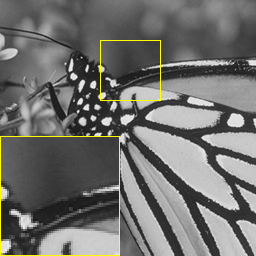
\includegraphics[width=0.18\linewidth]{2-9-1}  
	}\hspace{-0.02\linewidth}
	\subfigure[noisy image/20.17dB]{   
		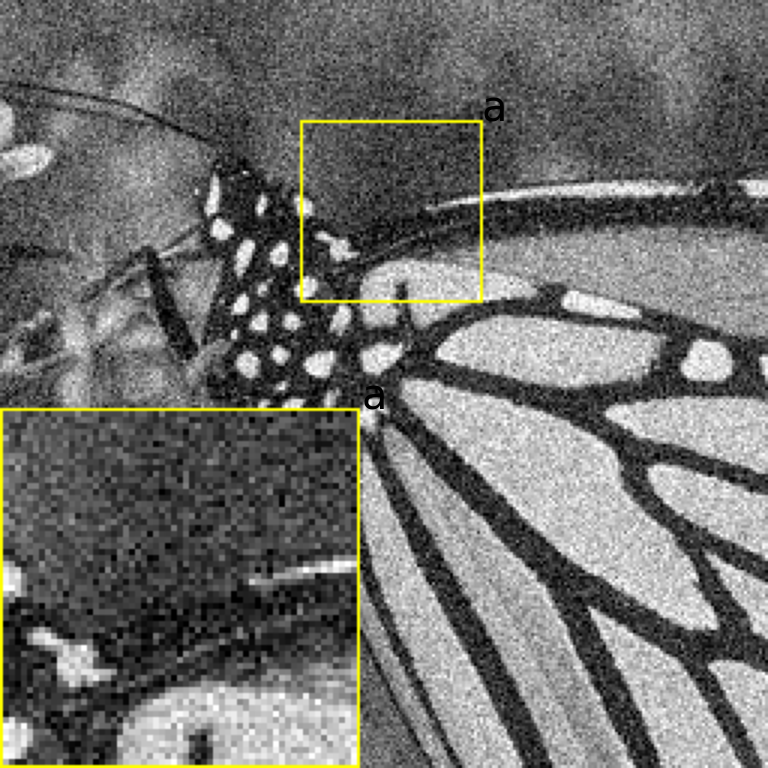
\includegraphics[width=0.18\linewidth]{2-9-2}  
	}\hspace{-0.02\linewidth}
	\subfigure[BM3D/29.39dB]{   
		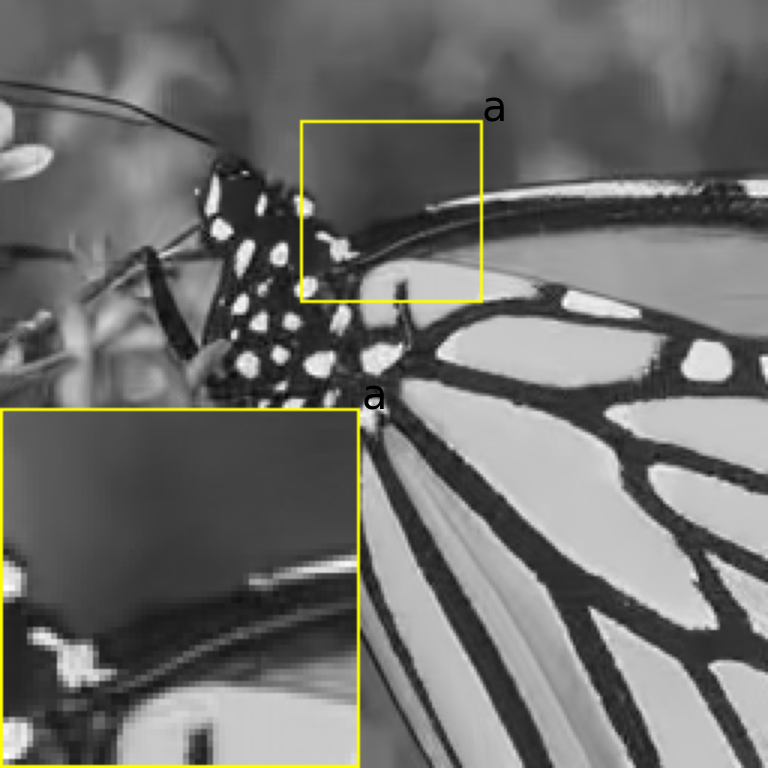
\includegraphics[width=0.18\linewidth]{2-9-3}  
	} 
	\\
	\subfigure[DnCNN-S/\color{red}30.39dB]{   
		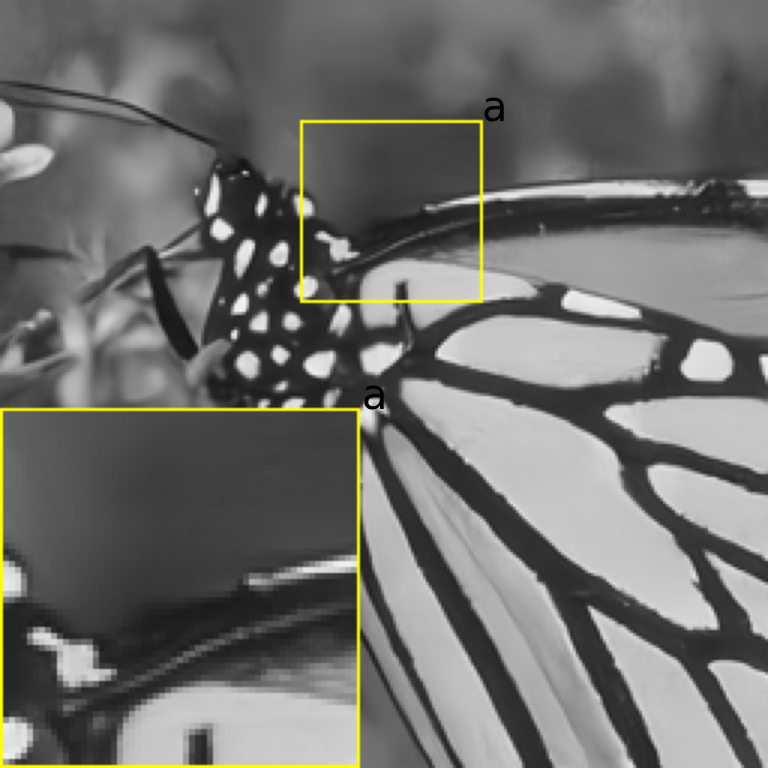
\includegraphics[width=0.18\linewidth]{2-9-4}  
	}\hspace{-0.02\linewidth}
	\subfigure[DnCNN-B/30.38dB]{   
		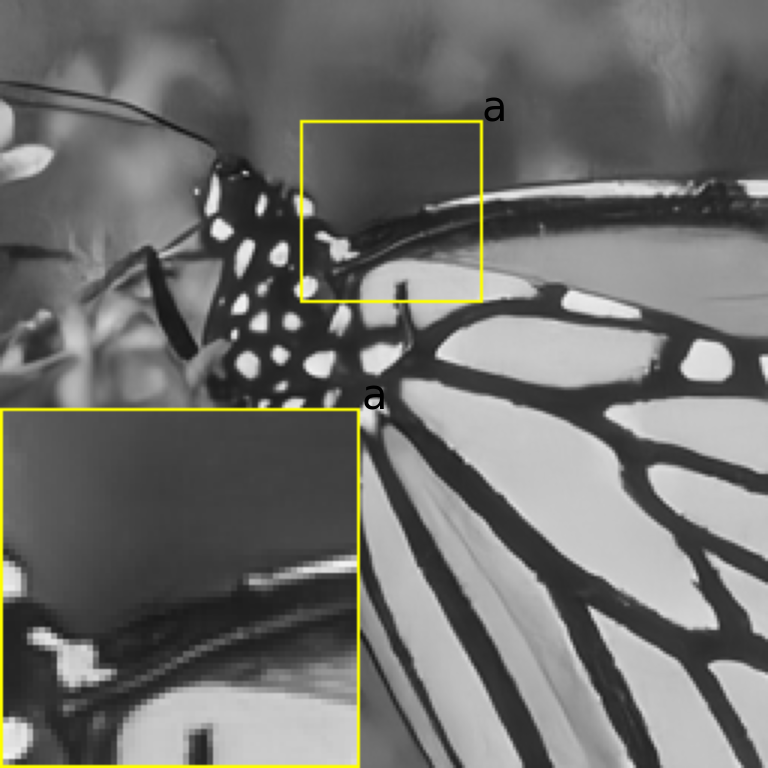
\includegraphics[width=0.18\linewidth]{2-9-5}  
	}\hspace{-0.02\linewidth}
	\subfigure[IRCNN-S/30.26dB]{   
		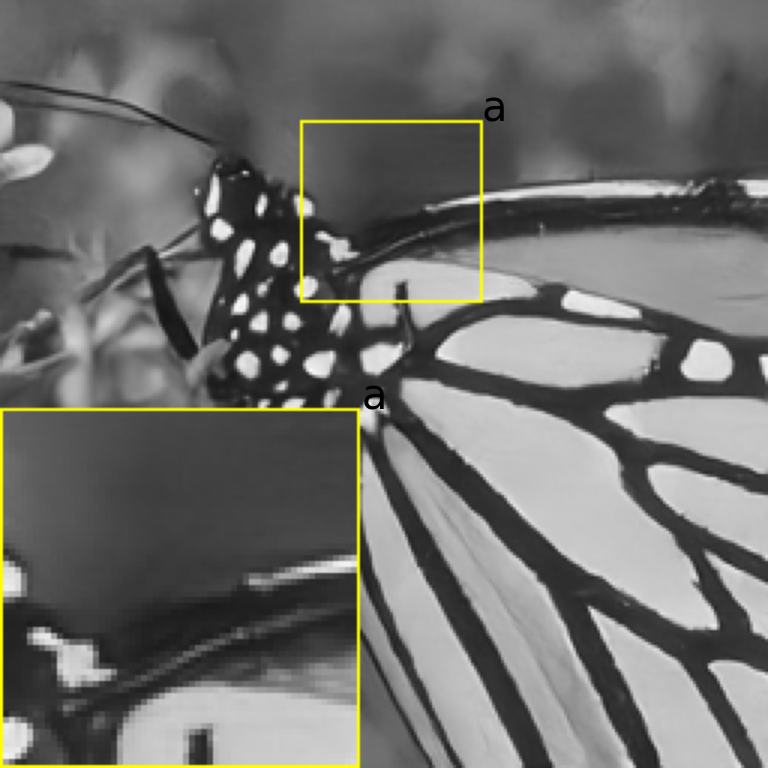
\includegraphics[width=0.18\linewidth]{2-9-6}  
	}\hspace{-0.02\linewidth}
	\subfigure[IRCNN-B/30.11dB]{   
		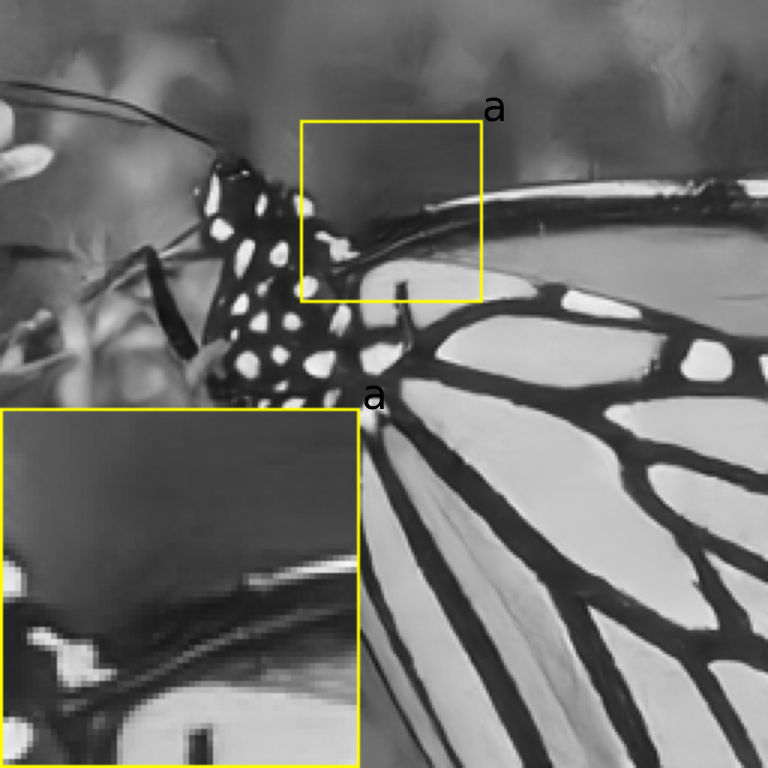
\includegraphics[width=0.18\linewidth]{2-9-7}  
	} 
	\caption{不同去噪算法的去噪效果图($\sigma=25$)} 
	\label{fig:2-9} 
\end{figure}
\begin{figure}[!htbp]
	\centering 
	\subfigure[original image]{
		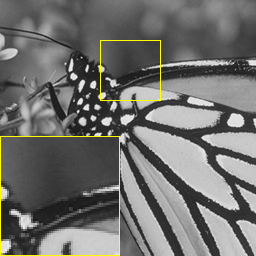
\includegraphics[width=0.18\linewidth]{2-10-1}  
	}\hspace{-0.02\linewidth}
	\subfigure[noisy image/20.17dB]{   
		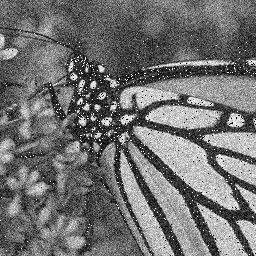
\includegraphics[width=0.18\linewidth]{2-10-2}  
	}\hspace{-0.02\linewidth}
	\subfigure[BM3D/29.39dB]{   
		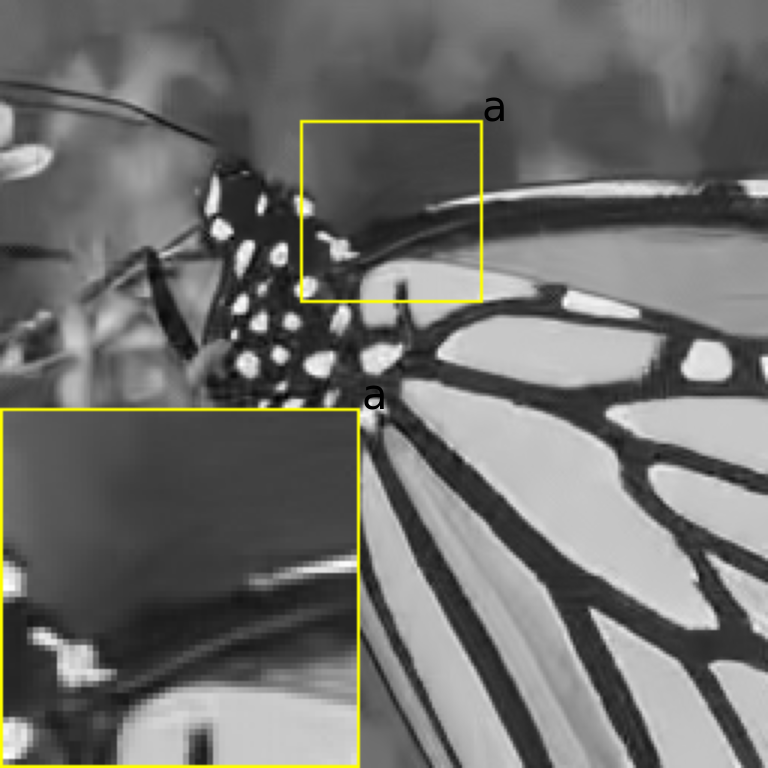
\includegraphics[width=0.18\linewidth]{2-10-3}  
	} 
	\\
	\subfigure[\tiny{realSN-DnCNN-S/30.37dB}]{   
		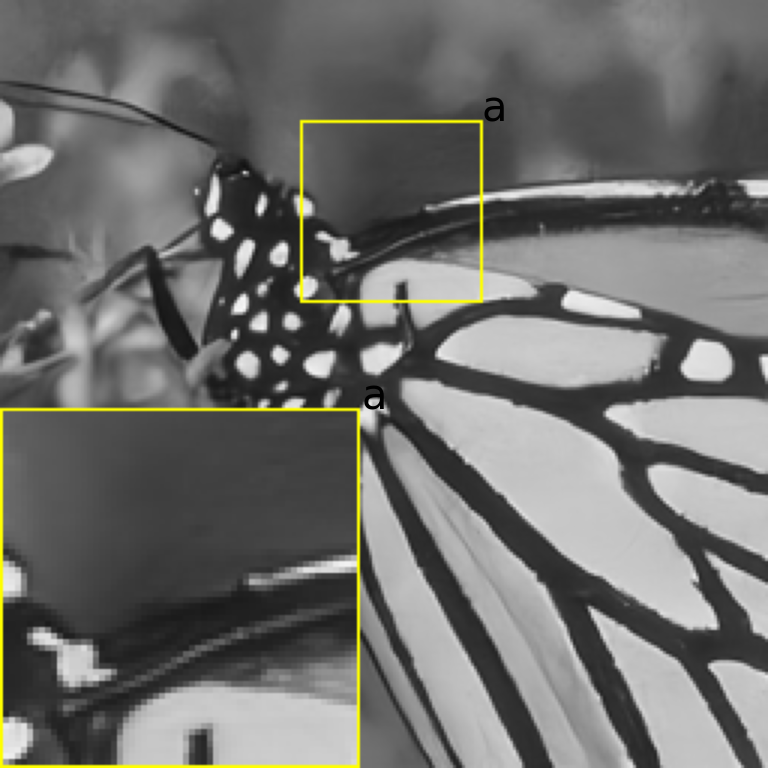
\includegraphics[width=0.18\linewidth]{2-10-4}  
	}\hspace{-0.02\linewidth}			
	\subfigure[\tiny{realSN-DnCNN-B/\color{red}30.38dB}]{   
		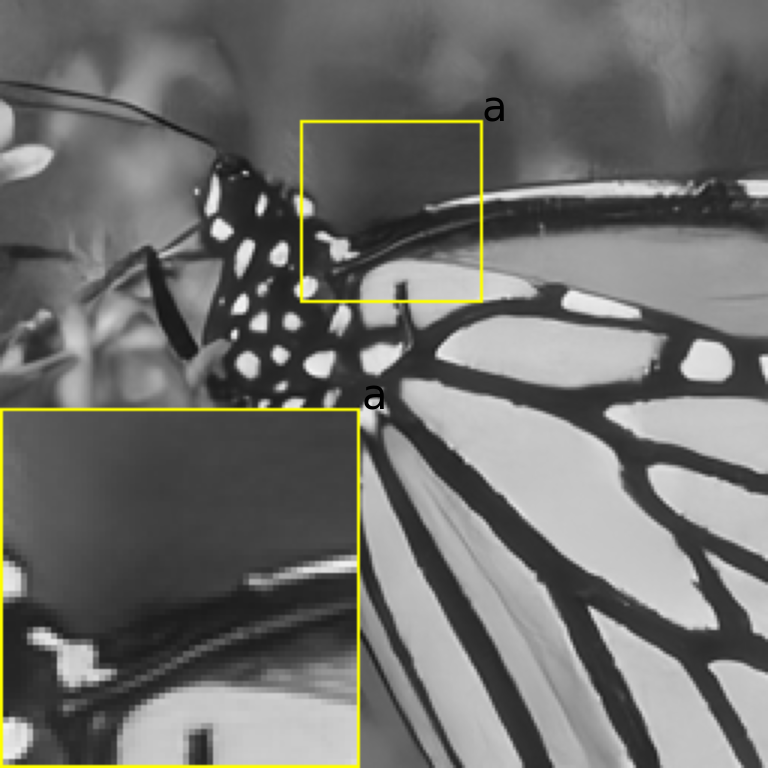
\includegraphics[width=0.18\linewidth]{2-10-5}  
	}\hspace{-0.02\linewidth}			
	\subfigure[\tiny{realSN-IRCNN-S/30.29dB}]{   
		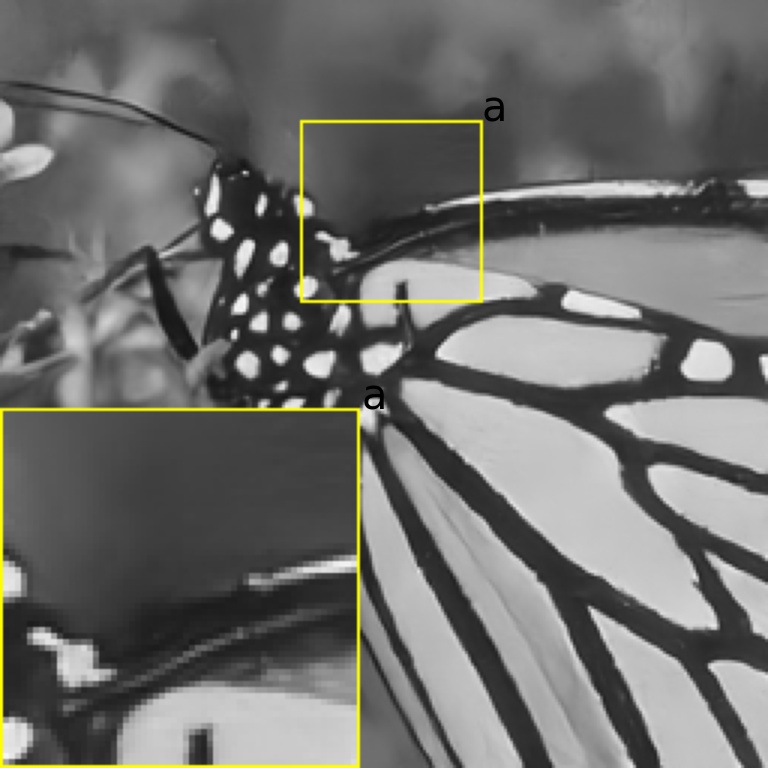
\includegraphics[width=0.18\linewidth]{2-10-6}  
	}\hspace{-0.02\linewidth}			
	\subfigure[\tiny{realSN-IRCNN-B/30.07dB}]{   
		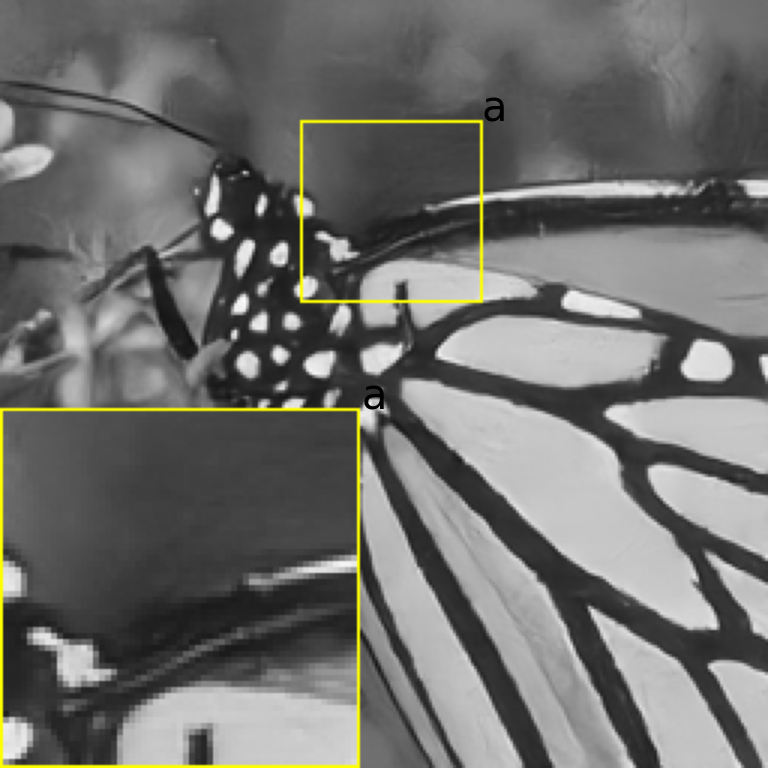
\includegraphics[width=0.18\linewidth]{2-10-7}
	}
	\caption{实谱归一化不同去噪算法的去噪效果图($\sigma=25$)}
	\label{fig:2-10}  
\end{figure}

从图\ref{fig:2-9}与图\ref{fig:2-10}可以出:(1)横向对比,从主观视觉的角度已无法区分各去噪图像的优劣,但基于深度学习的去噪算法在PSNR/SSIM上高于传统的BM3D算法,表明深度学习技术对于图像去噪任务的潜在优势,利用深度神经网络构造的去噪器取得当前SOTA结果;(2)纵向对比,基于实谱归一化的深度学习去噪器并未增强对盲高斯噪声的泛化能力,去噪效果与未加实谱归一化的原始去噪算法相当,引起这一现象原因为利普希茨约束导致欠拟合。因为神经网络利普希茨常数的估计较为复杂,现存的方法存在缺乏准确性或可伸缩性差等缺点,无法有效接近真实的全局利普希茨常数,只能在局部进行估计\supercite{Fazlyab}。故暂时无法确定实谱归一化是否真的起到了限制深度神经网络利普希茨常数的作用,留作日后研究。
%\begin{figure}[!hptb]
%	\centering
%	\begin{minipage}[t]{0.5\linewidth}
%		\centering
%		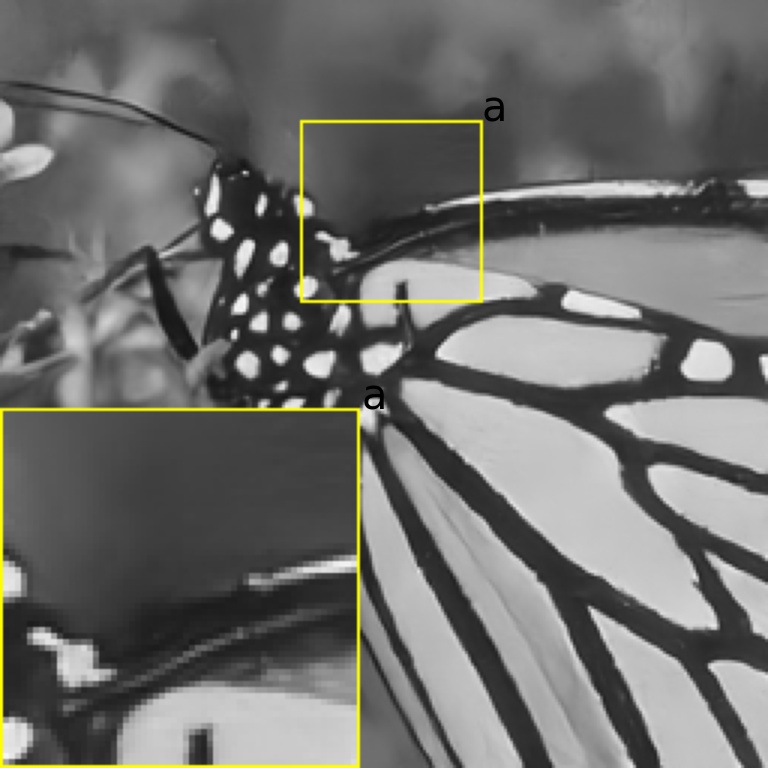
\includegraphics[width=\textwidth]{2-10-6}
%		\caption{text}
%	\end{minipage}%
%	\begin{minipage}[t]{0.5\textwidth}
%		\centering
%		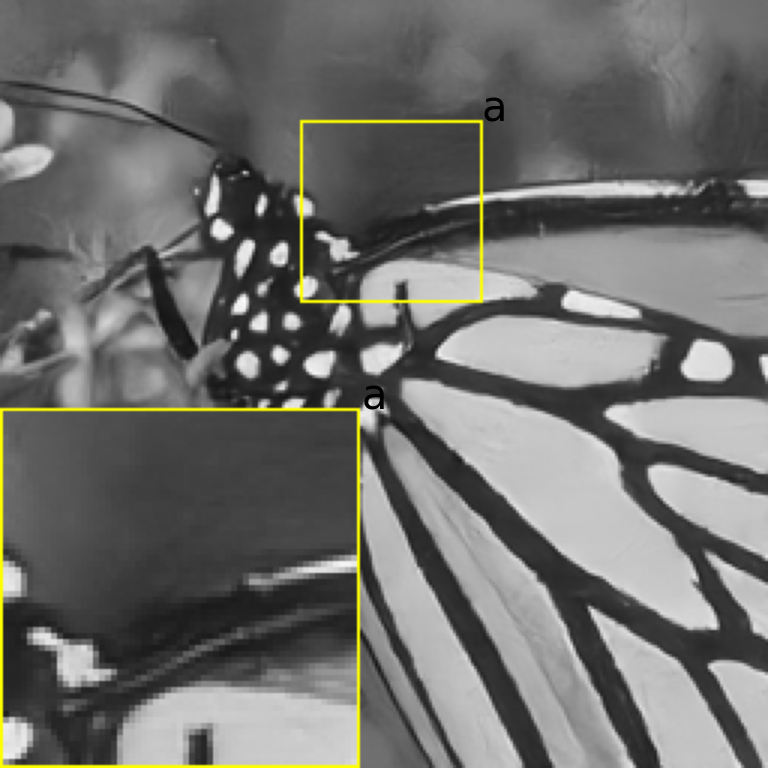
\includegraphics[width=\textwidth]{2-10-7}
%	\end{minipage}
%	\caption{两个并排图形}\label{fig-dbfig}
%\end{figure}

\subsection{TACE及其对比算法参数设置}
本章采用的测试数据集TestImages来自文献[10],共包含六张自然图像与六张非自然图像。在编码衍射系统设置中,本章采用随机空间光调制掩膜$M_i$,即复平面单位圆的随机均匀抽样,其如图\ref{fig:3-4}所示。此时它对应的观测矩阵为$A_{i}=FM_i,i\in[1,2,3,4]$,其中$F$表示二维快速傅里叶变换。故编码衍射模型表示为:
\begin{equation} \label{equation:3-22}
	y=\vert{Ax}\vert+\omega.
\end{equation}
其中$\omega$表示随机噪声。
\begin{figure}[!htbp]
	\centering
	\subfigure[$M_1$]{
		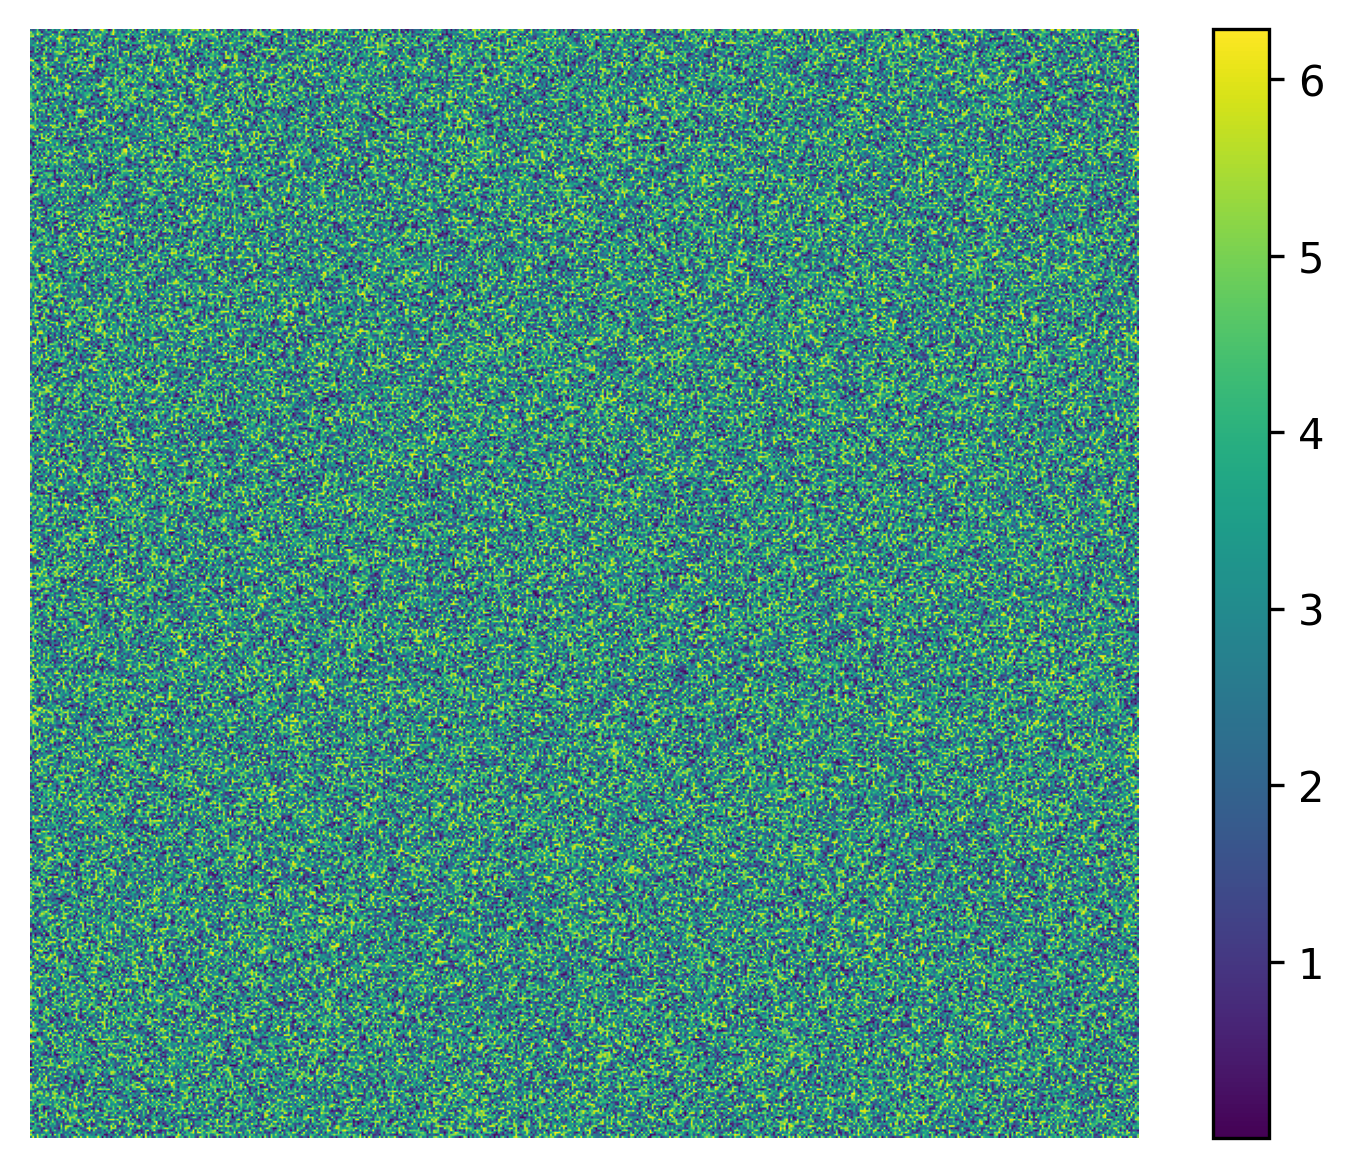
\includegraphics[width=0.2\linewidth]{barbara_slm_1}
	}\hspace{-0.0\linewidth}
	\subfigure[$M_2$]{
		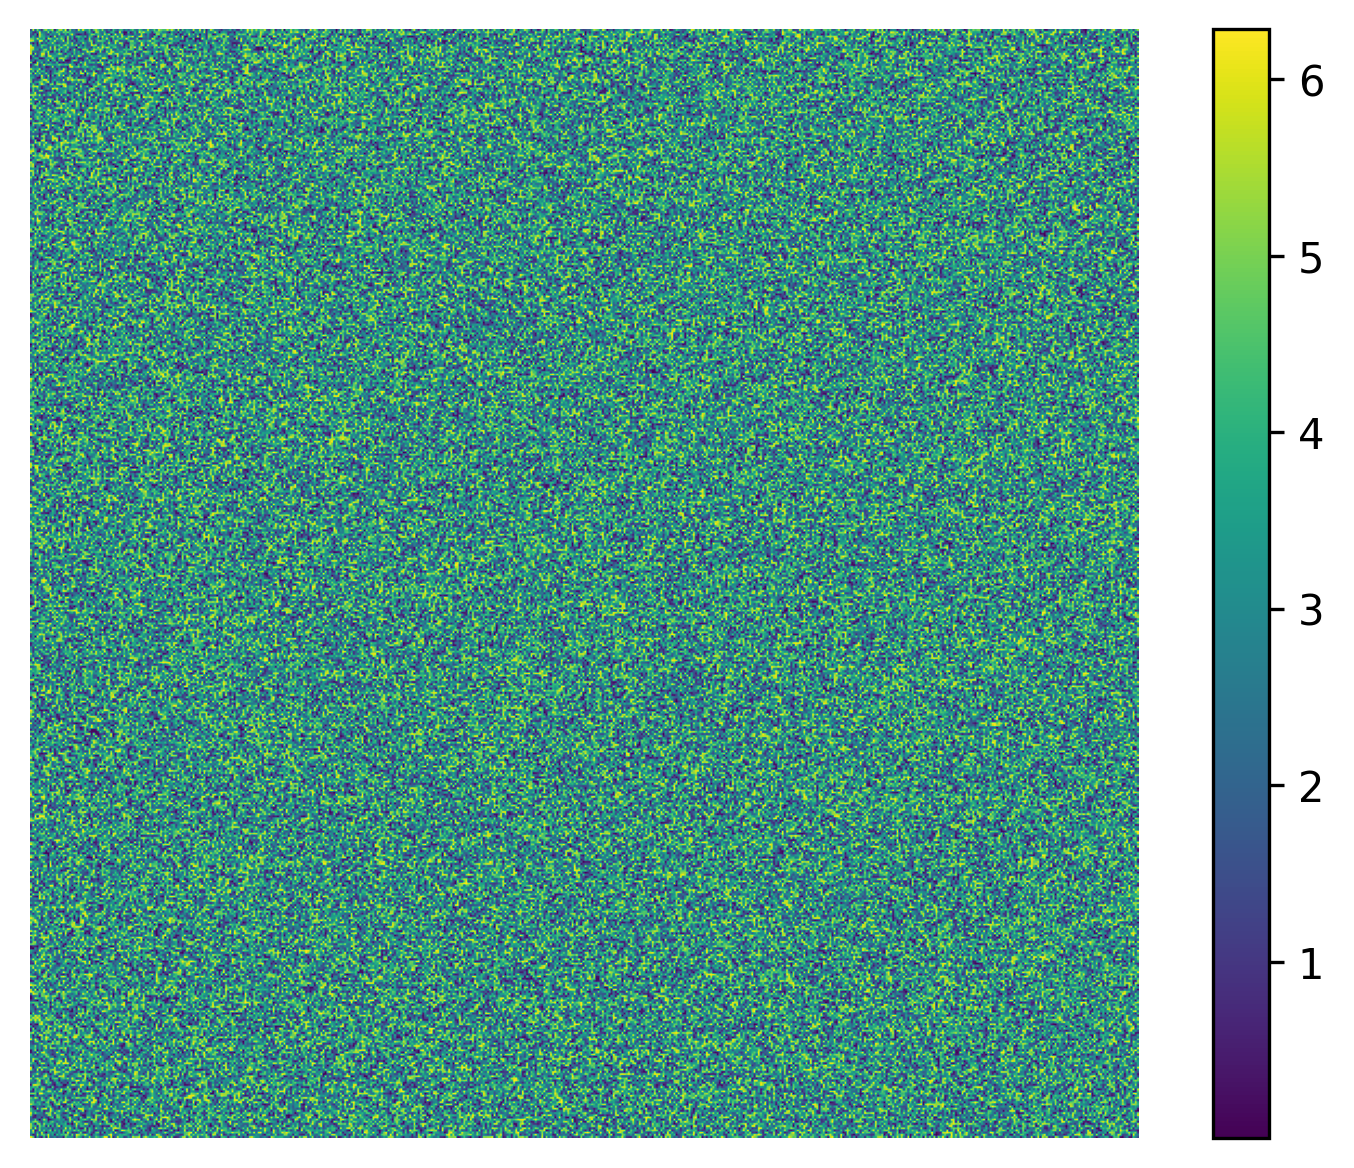
\includegraphics[width=0.2\linewidth]{barbara_slm_2}
	}\hspace{-0.0\linewidth}
	\subfigure[$M_3$]{
		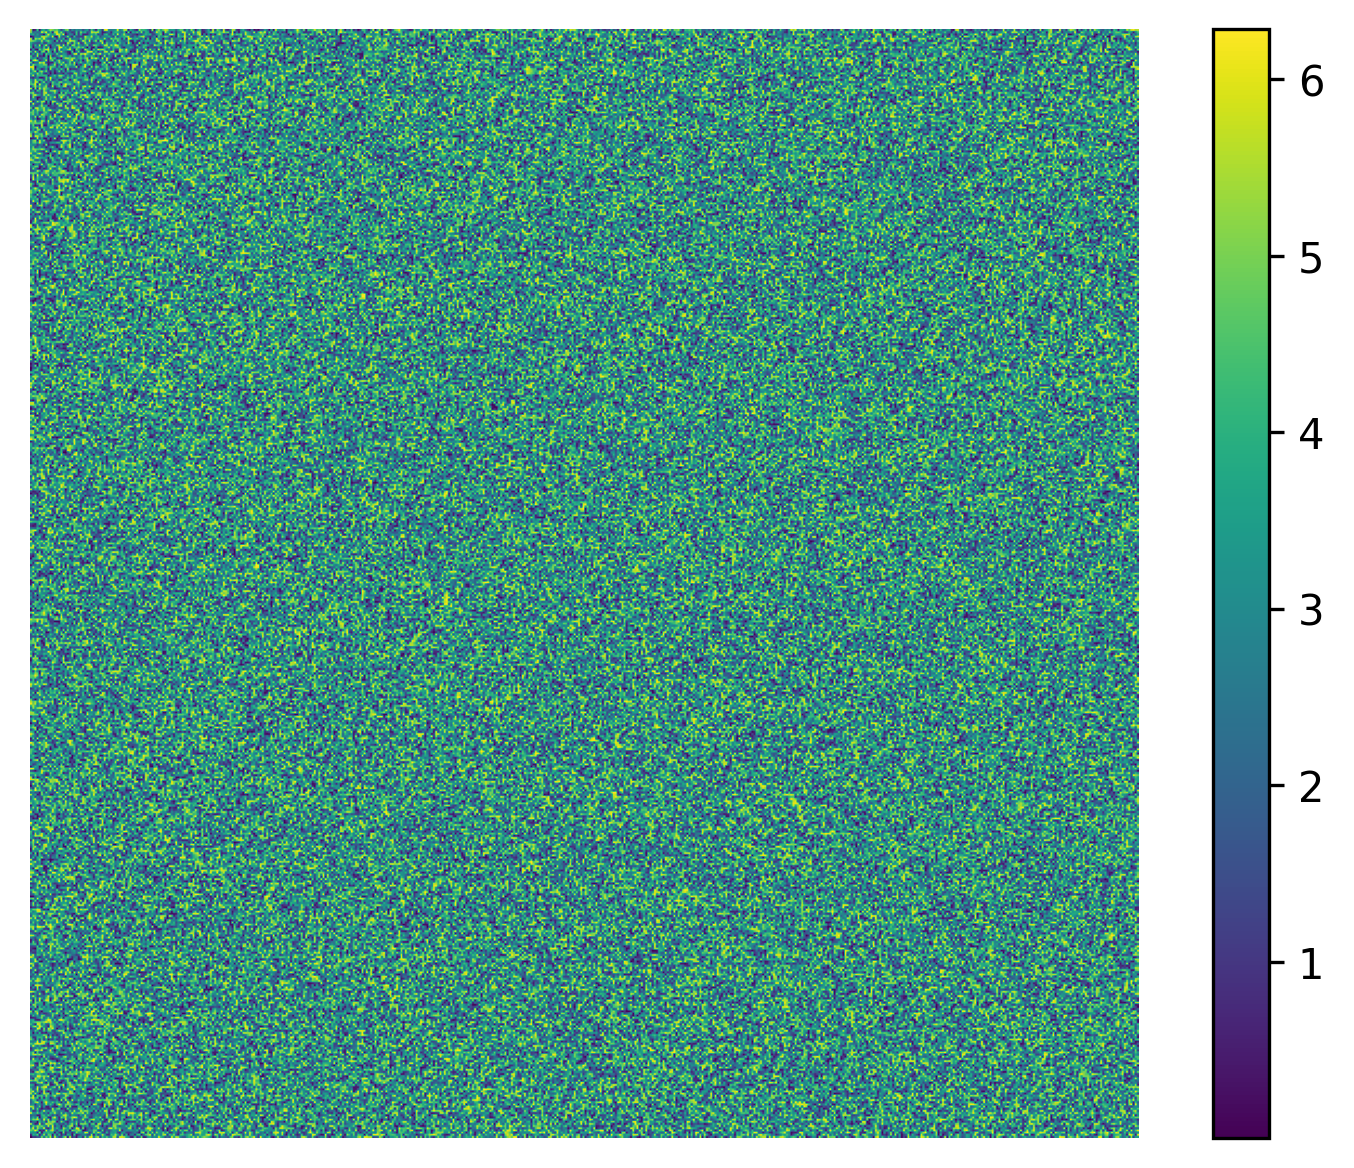
\includegraphics[width=0.2\linewidth]{barbara_slm_3}
	}\hspace{-0.0\linewidth}
	\subfigure[$M_4$]{
		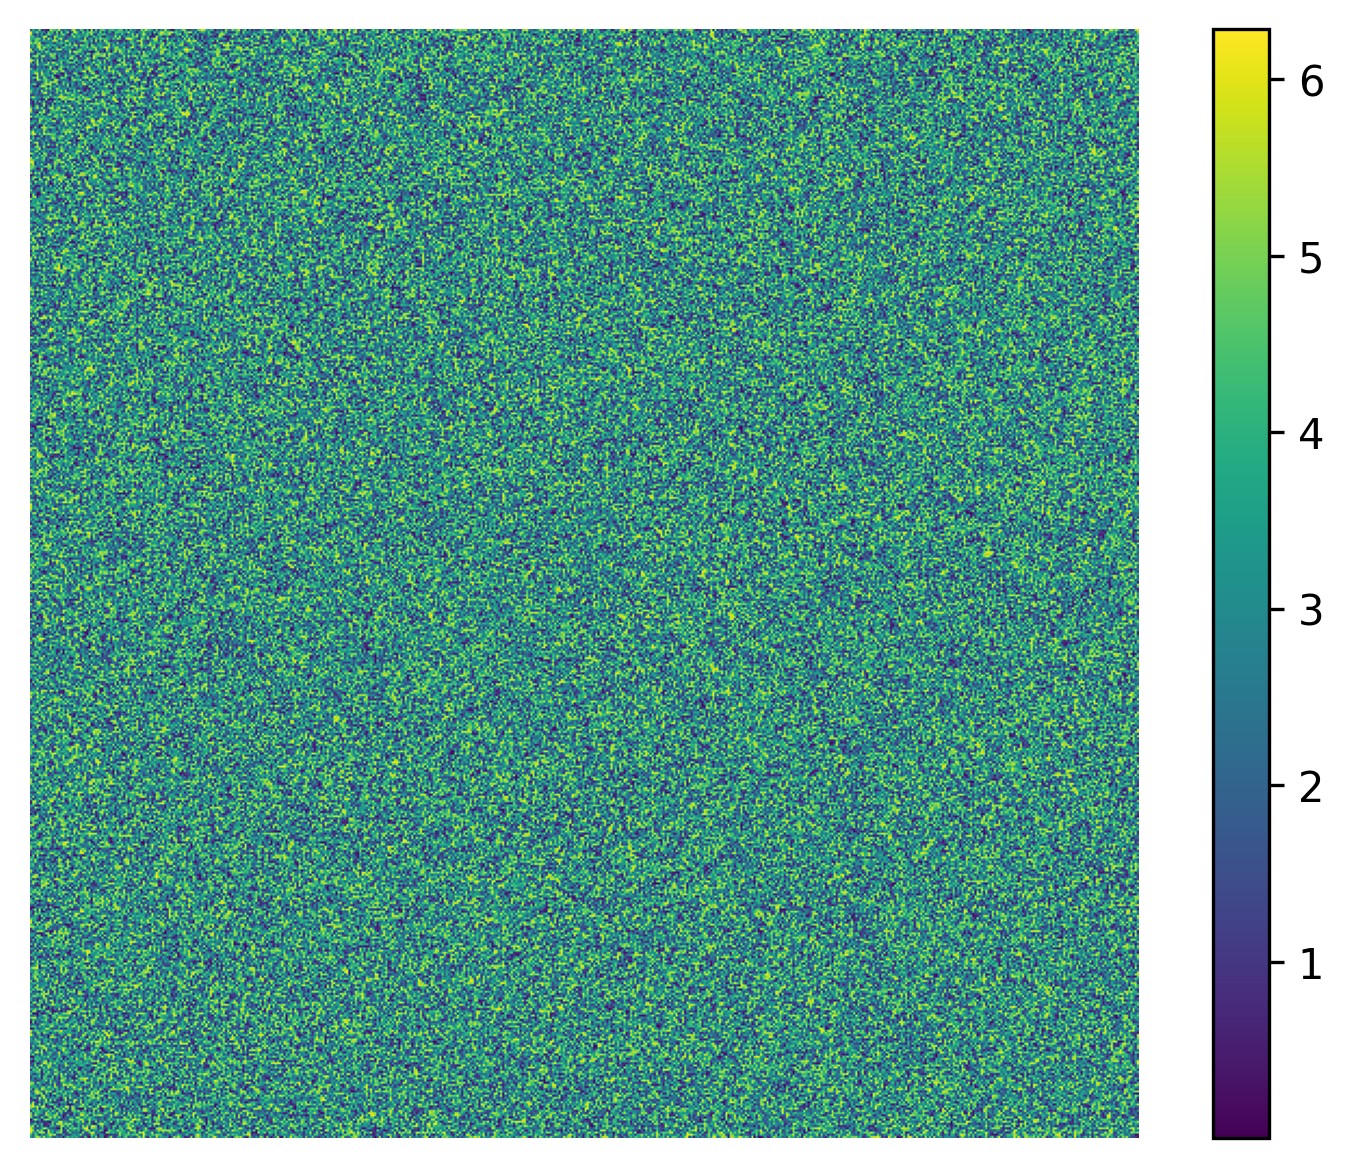
\includegraphics[width=0.2\linewidth]{barbara_slm_4}
	}
	\caption{Phase-only SLM示意图}
	\label{fig:3-4}
\end{figure}

在以下所有仿真实验中,随机SLM均设置相同的随机种子,以保证输入测试用例一致。此外,为了验证本文算法的有效性,本章针对不同噪声类型与噪声水平的观测值进行相位恢复仿真实验,并且从PSNR、SSIM和主观视觉角度对所提算法及其对比算法进行客观评价。

为了保证对比的公平性,算法\ref{algorithm:3-1}、\ref{algorithm:3-2}、\ref{algorithm:3-3}与peDeep均采用同一盲去噪器($\sigma=1\sim{50}$)。算法\ref{algorithm:3-1}、\ref{algorithm:3-2}、\ref{algorithm:3-3}根据默认值设置参数,prDeep利用FASTA的默认设置。另外,所有算法的初始值服从均匀分布。

\subsection{抗高斯噪声模型}
当式\eqref{equation:3-22}中的$\omega\sim{\mathcal{N}(0,\sigma^2\mathbf{I})}$时,观测值受高斯噪声的污染。相应的信噪比(SNR)定义为:
\begin{equation} \label{equation:3-23}
	\text{SNR}(\hat{y},y)=20\log_{10}{\frac{\Vert{y}\Vert_2}{\Vert{y-\hat{y}}\Vert_2}}.
\end{equation}
其中$\hat{y}$表示含噪观测值,$y$表示真实图像。表\ref{table:3-4}与表\ref{table:3-5}给出了不同噪声强度、不同去噪算子下四种算法重构原始图像的PSNR/SSIM结果。
\begin{table}[!htbp]
	\def\arraystretch{1.4}\centering\zihao{5}
	\caption{不同算法在DnCNN下获得平均PSNR(dB)/SSIM比较}
	\label{table:3-4}
	\begin{tabular*}{\linewidth}{@{}@{\extracolsep{\fill}}ccccc@{}}
		\toprule	%\multirow{2}*{算法}
		算法	& prDeep & PnP-ADMM & PnP-FBS & TACE \\
		%\cmidrule(r){2-5}
		\midrule
		$\text{SNR}=15$        & 32.37/0.8426   & 34.29/0.9003  & {\color{red}34.40}/0.8939 & 34.31/{\color{red}0.9005}  \\
		$\text{SNR}=20$        & 33.39/0.8387   &37.00/{\color{red}0.9392}  &{\color{red}37.11}/0.9345 & 36.98/0.9383  \\
		$\text{SNR}=25$        & 36.00/0.8907   & 39.60/{\color{red}0.9588}  & {\color{red}39.70}/0.9581 & 39.55/0.9567  \\
		\bottomrule
	\end{tabular*}
\end{table}
\begin{table}[!htbp]
	\def\arraystretch{1.4}\centering\zihao{5}
	\caption{不同算法在IRCNN下获得平均PSNR(dB)/SSIM比较}
	\label{table:3-5}
	\begin{tabular*}{\linewidth}{@{}@{\extracolsep{\fill}}ccccc@{}}
		\toprule
		算法	& prDeep & PnP-ADMM & PnP-FBS & TACE \\ %\cmidrule(r){2-5}
		\midrule
		$\text{SNR}=15$        & 32.25/0.8504   & 33.93/0.9050  & {\color{red}34.10}/{\color{red}0.9065} & 33.93/0.9035  \\
		$\text{SNR}=20$        & 33.20/0.8380   & 36.50/0.9364  & {\color{red}36.70}/{\color{red}0.9374} & 36.47/0.9347  \\
		$\text{SNR}=25$        & 35.99/0.8906   & 39.00/0.9562  & {\color{red}39.22}/{\color{red}0.9563} & 38.92/0.9531  \\
		\bottomrule
	\end{tabular*}
\end{table}

从表\ref{table:3-4}与表\ref{table:3-5}可以看出,TACE算法的重构图像质量优于prDeep算法,并且与PnP-ADMM算法结果接近,验证了PnP-ADMM与TACE收敛到相同的不动点。由于PnP-FBS使用了自适应迭代步长技术,使得该算法为SOTA结果。再者TACE算法有着明确的优化方程,故在理论上可以分析其收敛性与收敛速度。而PnP-ADMM和PnP-FBS没有明确的优化问题,为非凸框架,分析收敛性依赖于对去噪算子的假设。

为衡量算法的计算复杂度,表\ref{table:3-6}给出了四种算法在同一测试集上的GPU平均运行时间。从表\ref{table:3-6}可以看出TACE算法的运行时间与即插即用算法比较接近,并没有出现过大的数量级差距。并且这是算法的绝对运行时间,可比较性存在争议。
\begin{table}[!htbp]
	\def\arraystretch{1.4}\centering\zihao{5}
	\caption{不同算法不同去噪器在Barbara上的运行时间(s)(SNR=25dB)}
	\label{table:3-6}
	\begin{tabular*}{\linewidth}{@{}@{\extracolsep{\fill}}ccccc@{}}
		\toprule
		算法	& prDeep & PnP-ADMM & PnP-FBS & TACE \\ %\cmidrule(r){2-5}
		\midrule
	    512x512 & 27.92/{\color{blue}8.70}   & {\color{blue}25.74}/9.64  & 28.43/9.46 & 30.56/10.58 \\
	    Device	         & GPU   & GPU  & GPU	& GPU \\
		\bottomrule
	\end{tabular*}
\end{table}

图\ref{fig:3-6}与图\ref{fig:3-7}给出了不同算法在DnCNN和IRCNN去噪算子下当SNR=15dB时Barbara与Pollen的重构结果。从图\ref{fig:3-6}与图\ref{fig:3-7}可以看出TACE算法与对比算法已经无法从主观视觉上区别重构图像的优劣。但在PSNR的角度,两阶段TACE算法并没有取得SOTA的结果,这是因为TACE算法与PnP-ADMM算法不动点的等价性。
\begin{figure}[!htbp]
	\centering
	\subfigure[Original]{
		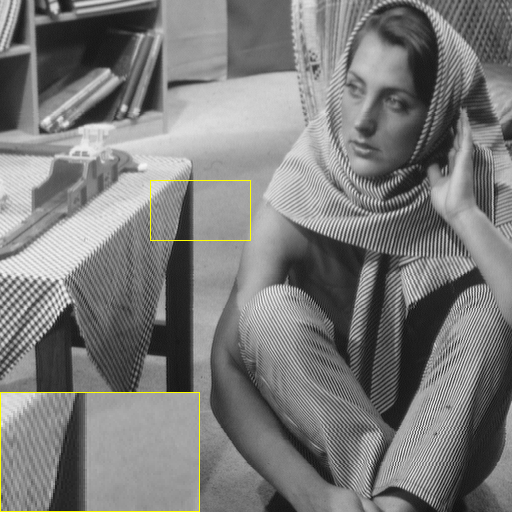
\includegraphics[width=0.18\linewidth]{3-6-1}
	}\hspace{-0.01\linewidth}
	\subfigure[prDeep/31.10]{
		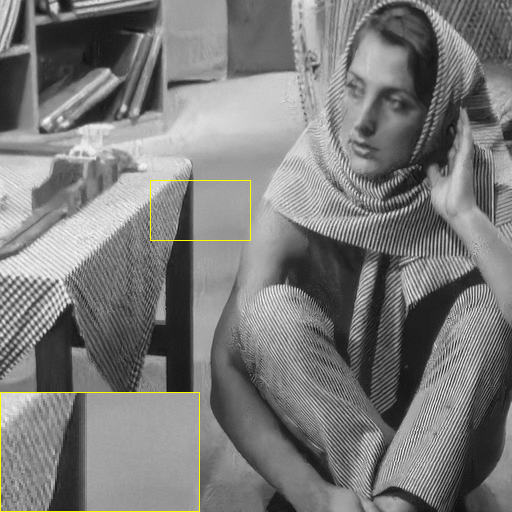
\includegraphics[width=0.18\linewidth]{3-6-2}
	}\hspace{-0.01\linewidth}
	\subfigure[PnP-ADMM/31.36]{
		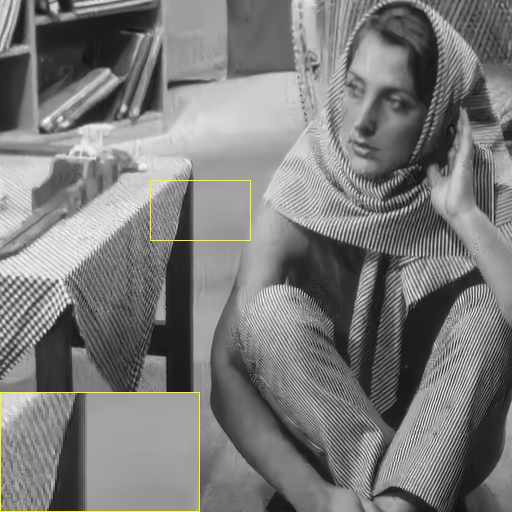
\includegraphics[width=0.18\linewidth]{3-6-3}
	}\hspace{-0.01\linewidth}
	\subfigure[PnP-FBS/{\color{red}31.51}]{
		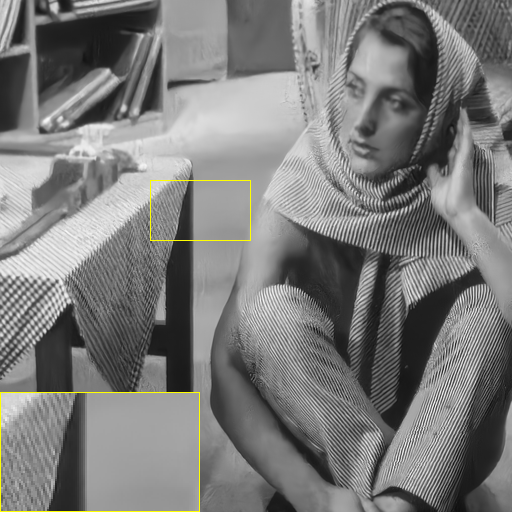
\includegraphics[width=0.18\linewidth]{3-6-4}
	}\hspace{-0.01\linewidth}
	\subfigure[TACE/31.43]{
		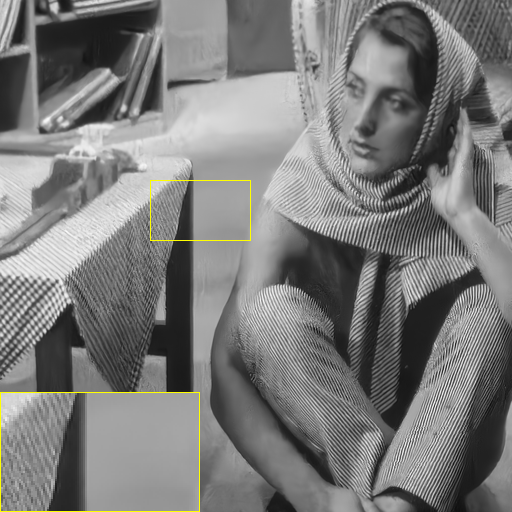
\includegraphics[width=0.18\linewidth]{3-6-5}
	}
	
	\subfigure[Original]{
		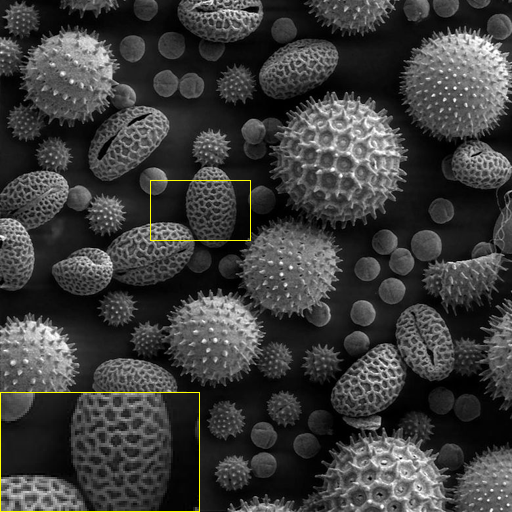
\includegraphics[width=0.18\linewidth]{3-6-6}
	}\hspace{-0.01\linewidth}
	\subfigure[prDeep/31.24]{
		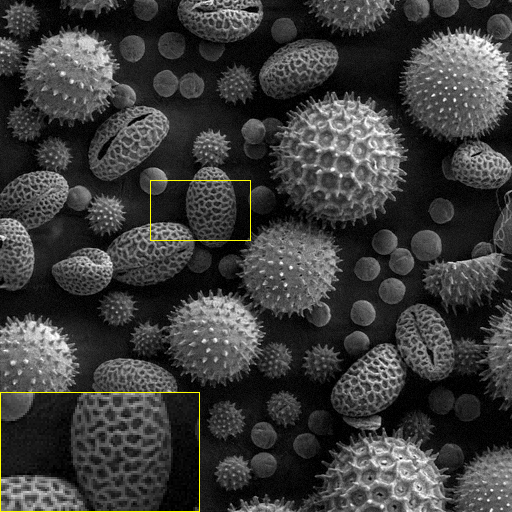
\includegraphics[width=0.18\linewidth]{3-6-7}
	}\hspace{-0.01\linewidth}
	\subfigure[PnP-ADMM/32.90]{
		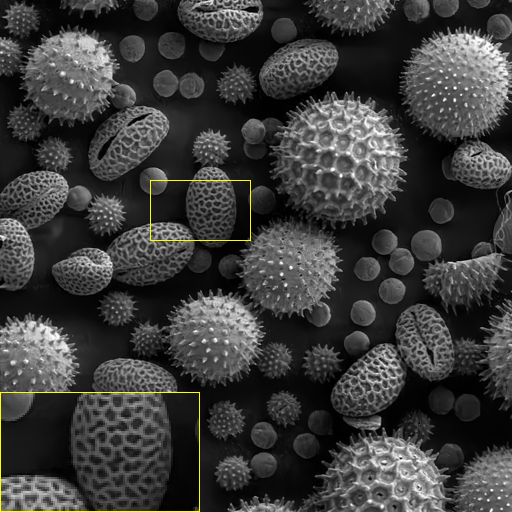
\includegraphics[width=0.18\linewidth]{3-6-8}
	}\hspace{-0.01\linewidth}
	\subfigure[PnP-FBS/{\color{red}33.01}]{
		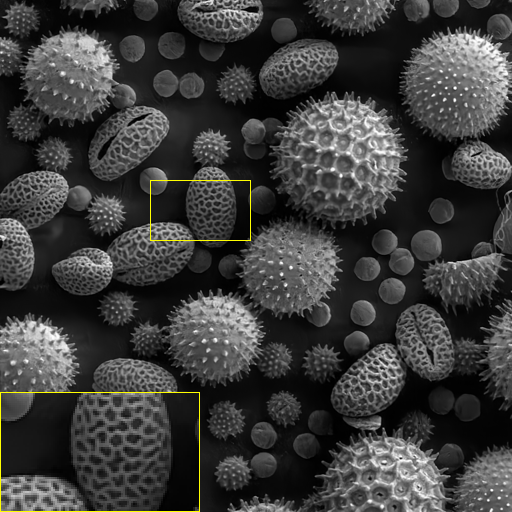
\includegraphics[width=0.18\linewidth]{3-6-9}
	}\hspace{-0.01\linewidth}
	\subfigure[TACE/32.92]{
		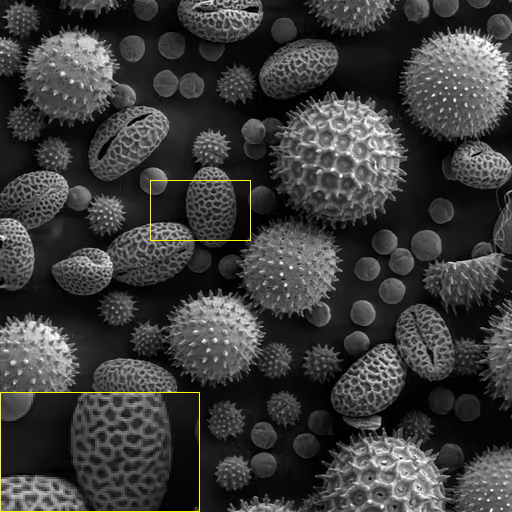
\includegraphics[width=0.18\linewidth]{3-6-10}
	}
	\caption{Barbara与Pollen重构结果(SNR=15dB,DnCNN)} 
	\label{fig:3-6}
\end{figure}
\begin{figure}[!htbp]
	\centering
	\subfigure[Original]{
		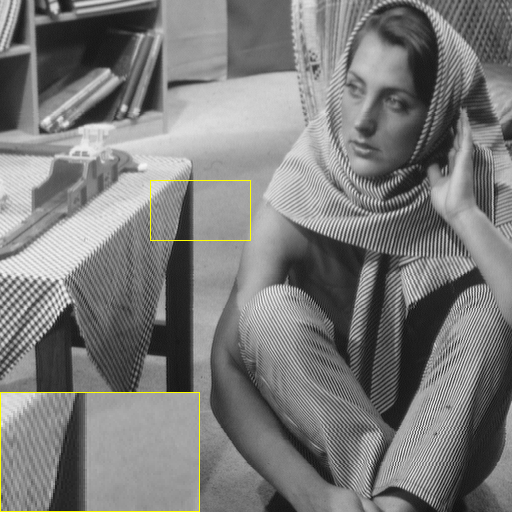
\includegraphics[width=0.18\linewidth]{3-7-1}
	}\hspace{-0.01\linewidth}
	\subfigure[prDeep/30.38]{
		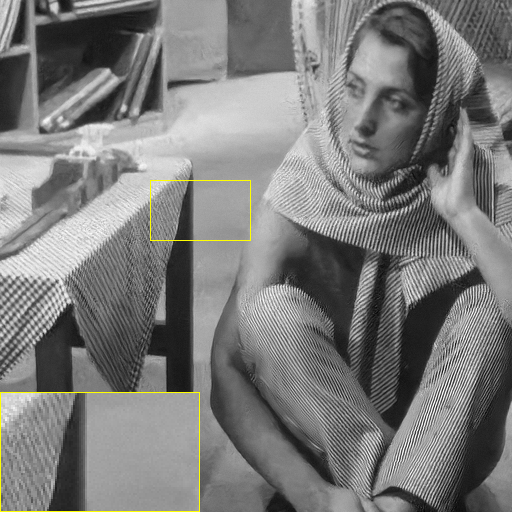
\includegraphics[width=0.18\linewidth]{3-7-2}
	}\hspace{-0.01\linewidth}
	\subfigure[PnP-ADMM/30.55]{
		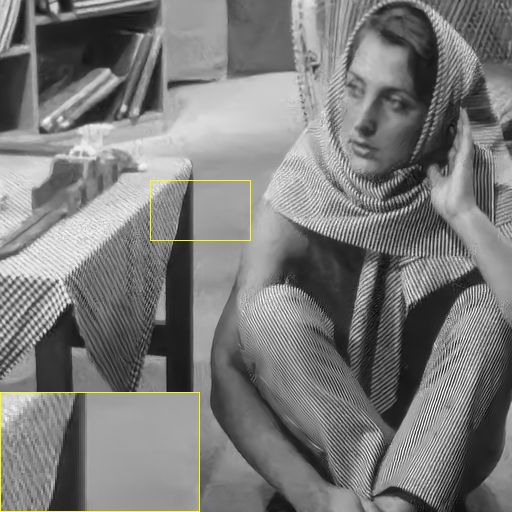
\includegraphics[width=0.18\linewidth]{3-7-3}
	}\hspace{-0.01\linewidth}
	\subfigure[PnP-FBS/{\color{red}31.00}]{
		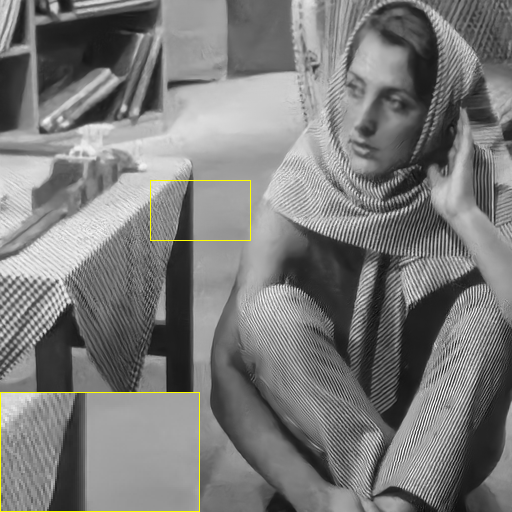
\includegraphics[width=0.18\linewidth]{3-7-4}
	}\hspace{-0.01\linewidth}
	\subfigure[TACE/30.60]{
		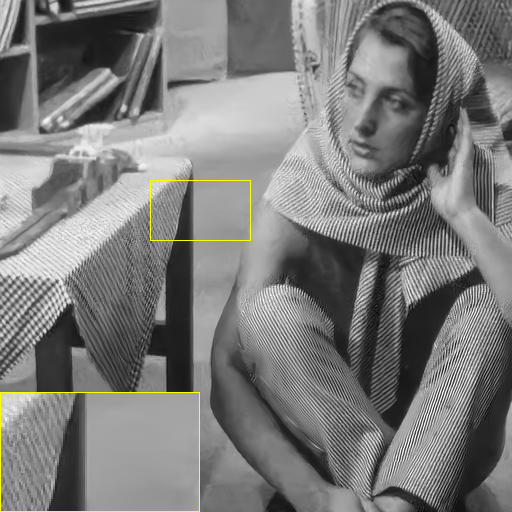
\includegraphics[width=0.18\linewidth]{3-7-5}
	}
	
	\subfigure[Original]{
		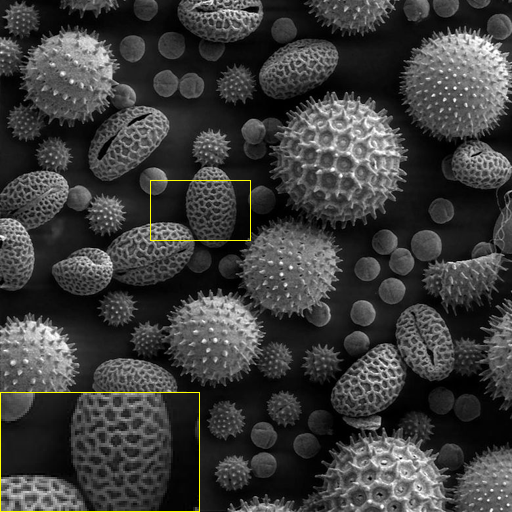
\includegraphics[width=0.18\linewidth]{3-7-6}
	}\hspace{-0.01\linewidth}
	\subfigure[prDeep/30.96]{
		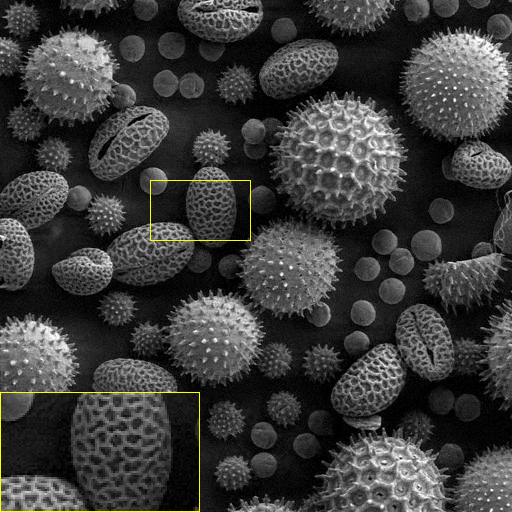
\includegraphics[width=0.18\linewidth]{3-7-7}
	}\hspace{-0.01\linewidth}
	\subfigure[PnP-ADMM/32.56]{
		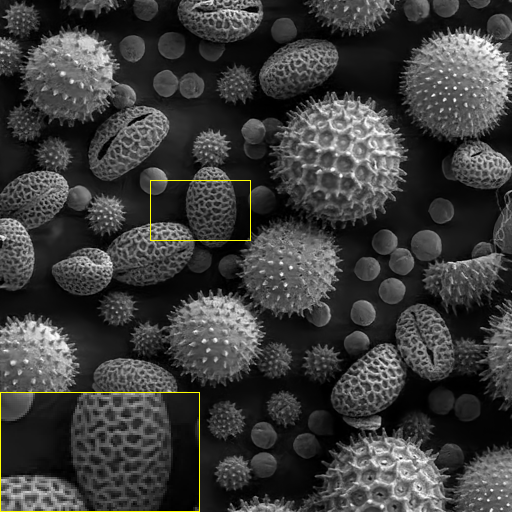
\includegraphics[width=0.18\linewidth]{3-7-8}
	}\hspace{-0.01\linewidth}
	\subfigure[PnP-FBS/{\color{red}32.72}]{
		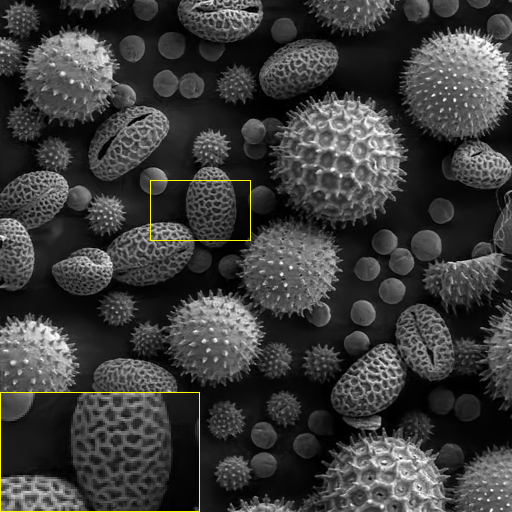
\includegraphics[width=0.18\linewidth]{3-7-9}
	}\hspace{-0.01\linewidth}
	\subfigure[TACE/32.58]{
		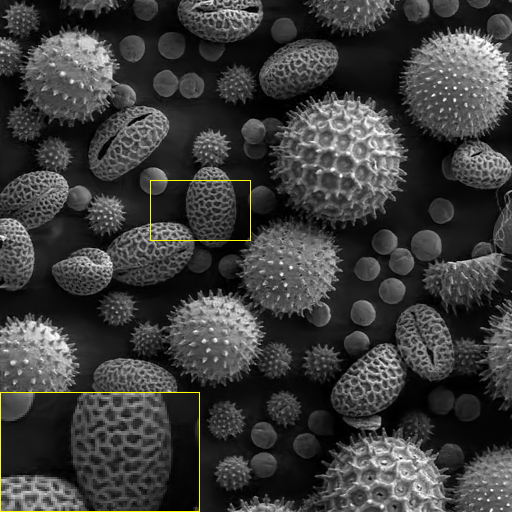
\includegraphics[width=0.18\linewidth]{3-7-10}
	}
	\caption{Barbara与Pollen重构结果(SNR=15dB,IRCNN)}
	\label{fig:3-7}
\end{figure}

为验证假设\ref{assumption:3-2},图\ref{fig:3-8}给出了PnP-ADMM与TACE算法各个代理在迭代过程中的利普希茨常数分布直方图,测试图像为Barbara,SNR=15dB,各个代理迭代过程中的利普希茨常数由定义\ref{def:3-1}计算。
\begin{figure}[!htbp]
	\centering
	\subfigure[\scriptsize PnP-ADMM(DnCNN)]{
		\label{subfigure:3-1-1}
		\begin{minipage}[b]{0.18\linewidth}
			\centering
			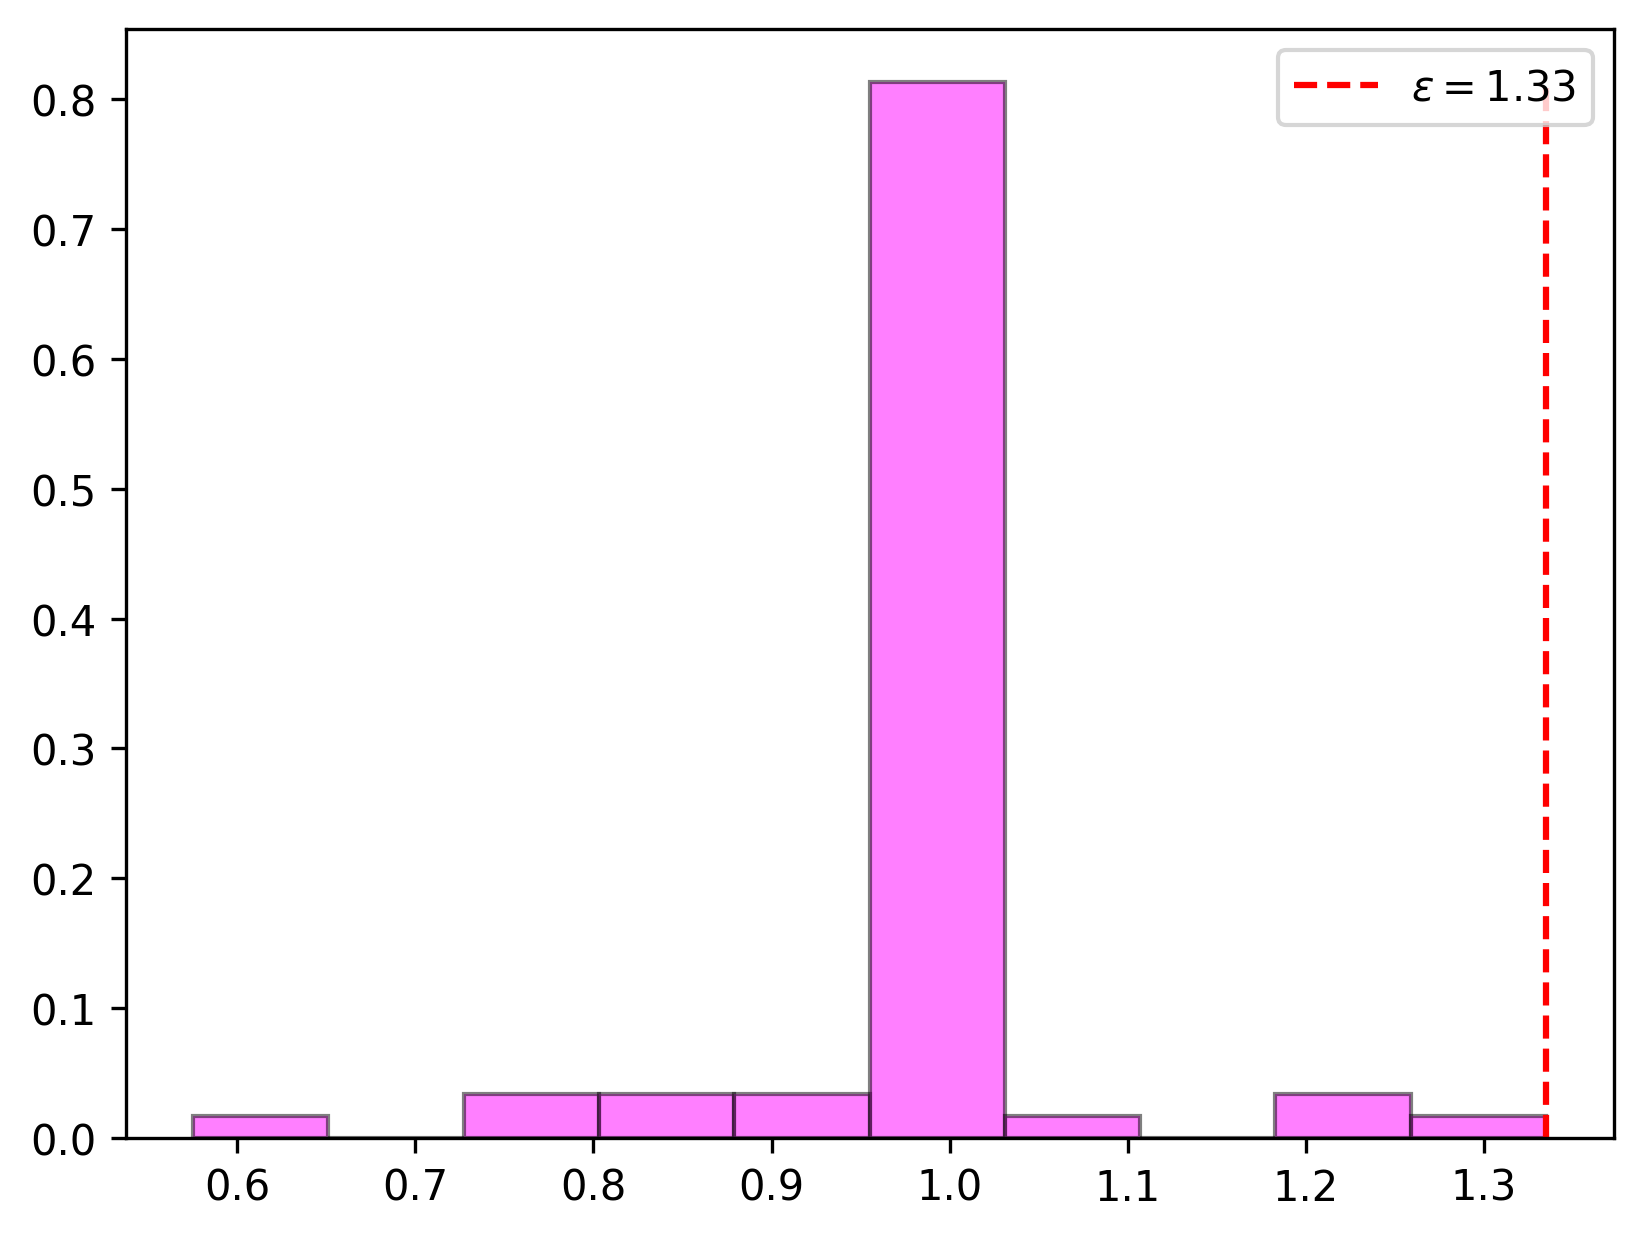
\includegraphics[width=\linewidth]{3-8-1}\\
			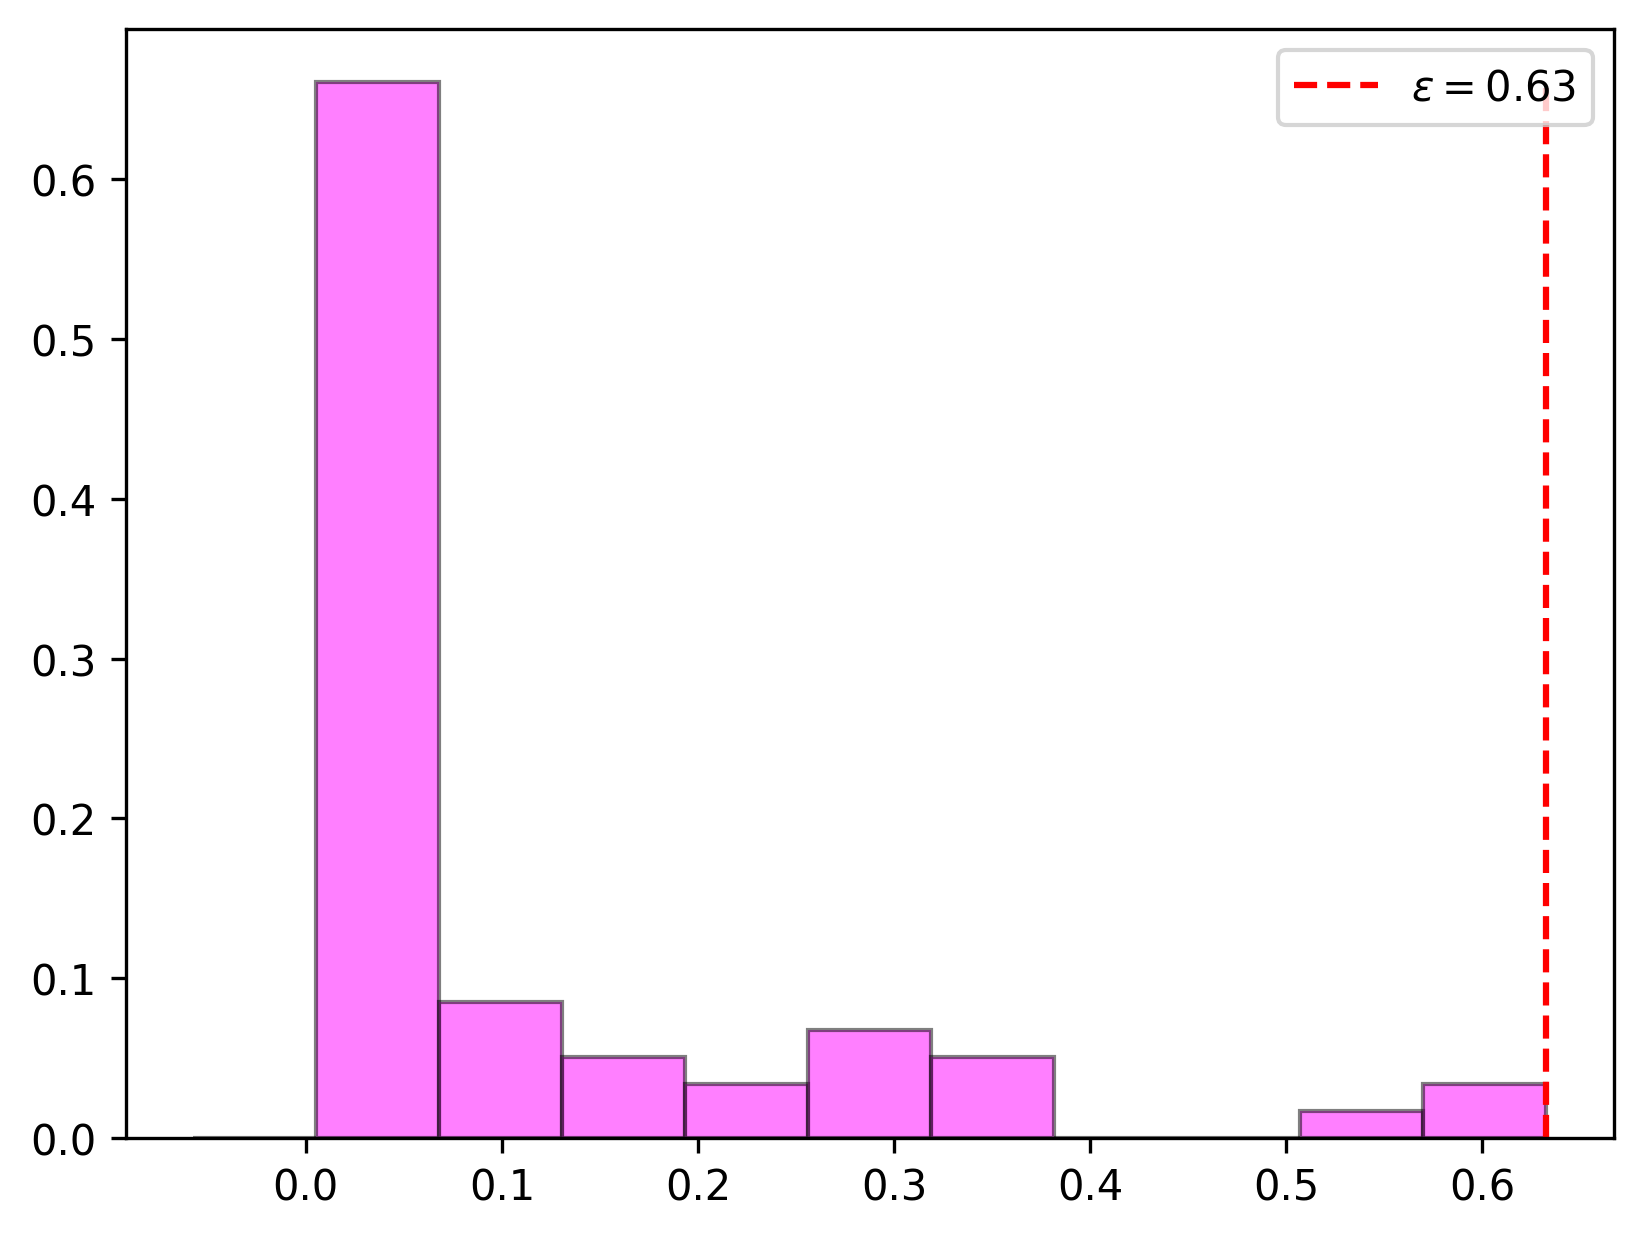
\includegraphics[width=\linewidth]{3-8-2}
			%\caption{fig}
		\end{minipage}
	}
	\subfigure[\scriptsize TACE(DnCNN)]{
		\label{subfigure:3-1-2}
		\begin{minipage}[b]{0.18\linewidth}
			\centering
			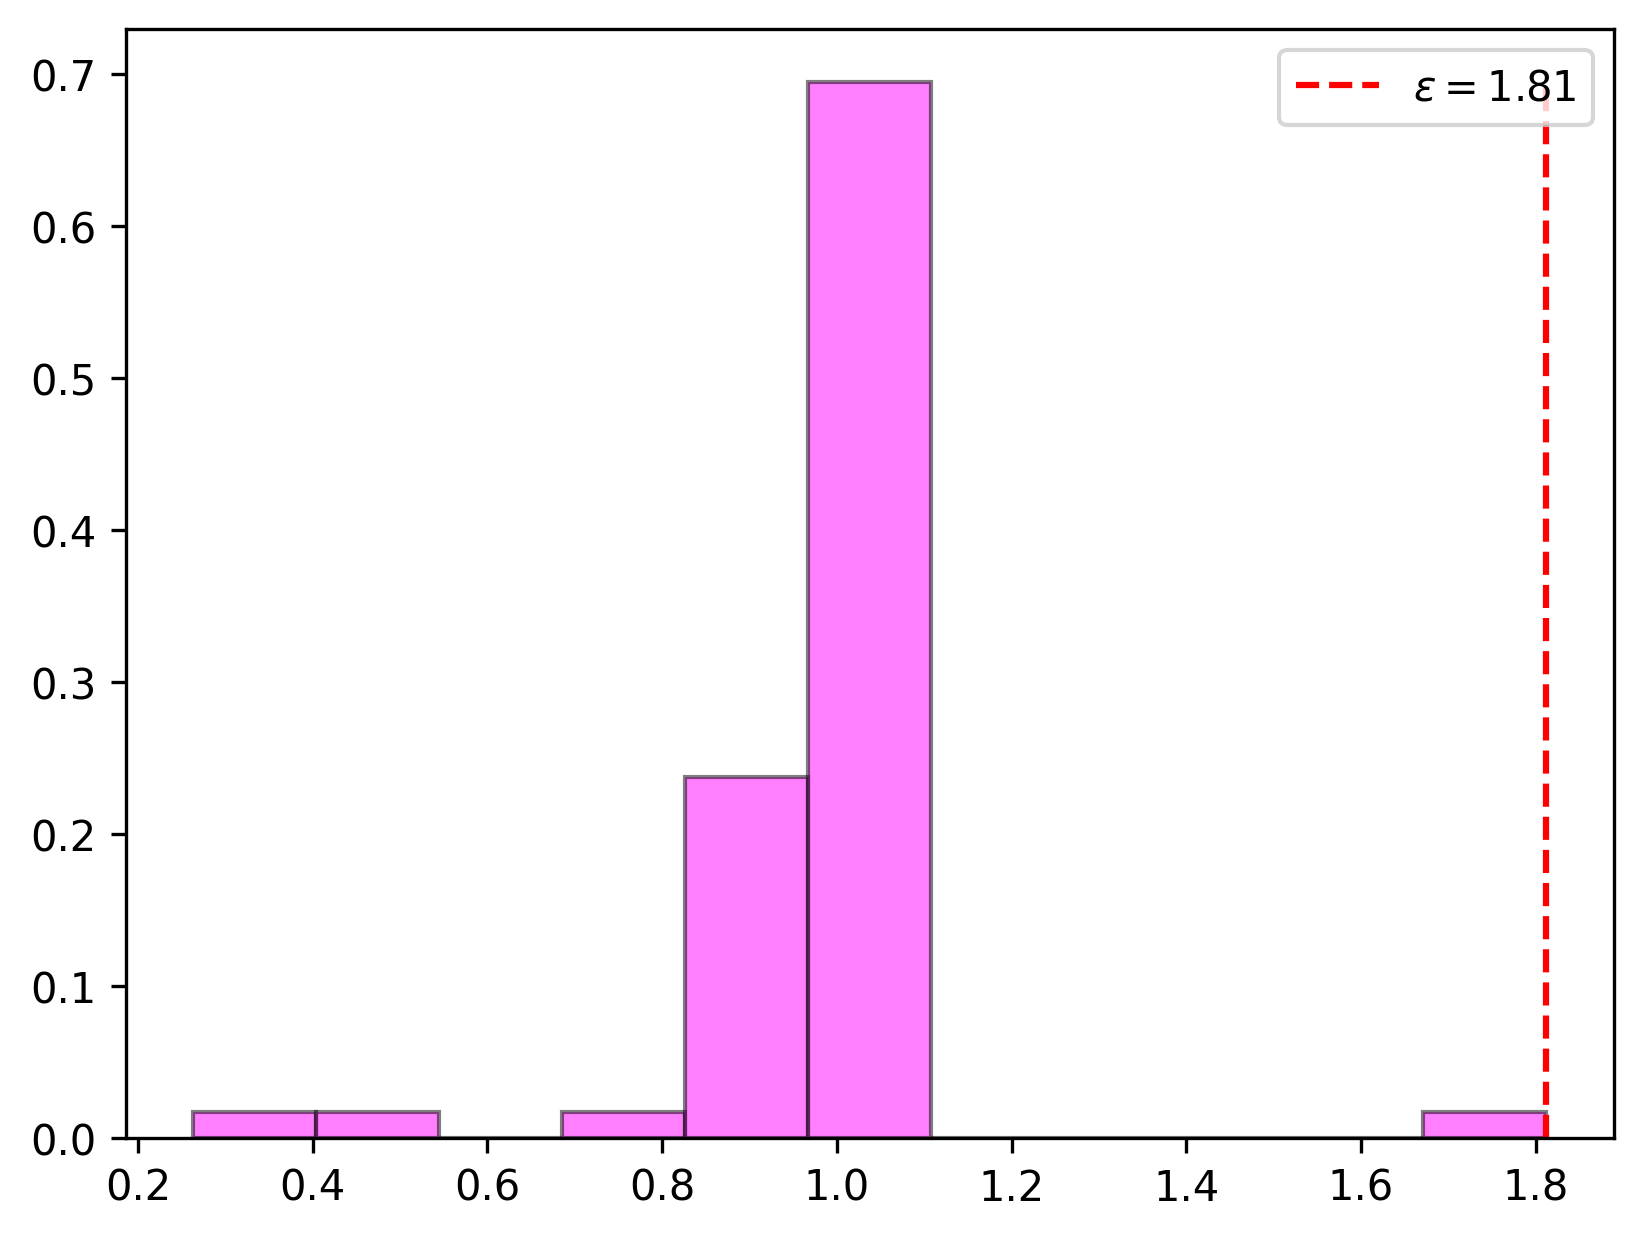
\includegraphics[width=\linewidth]{3-8-3}\\
			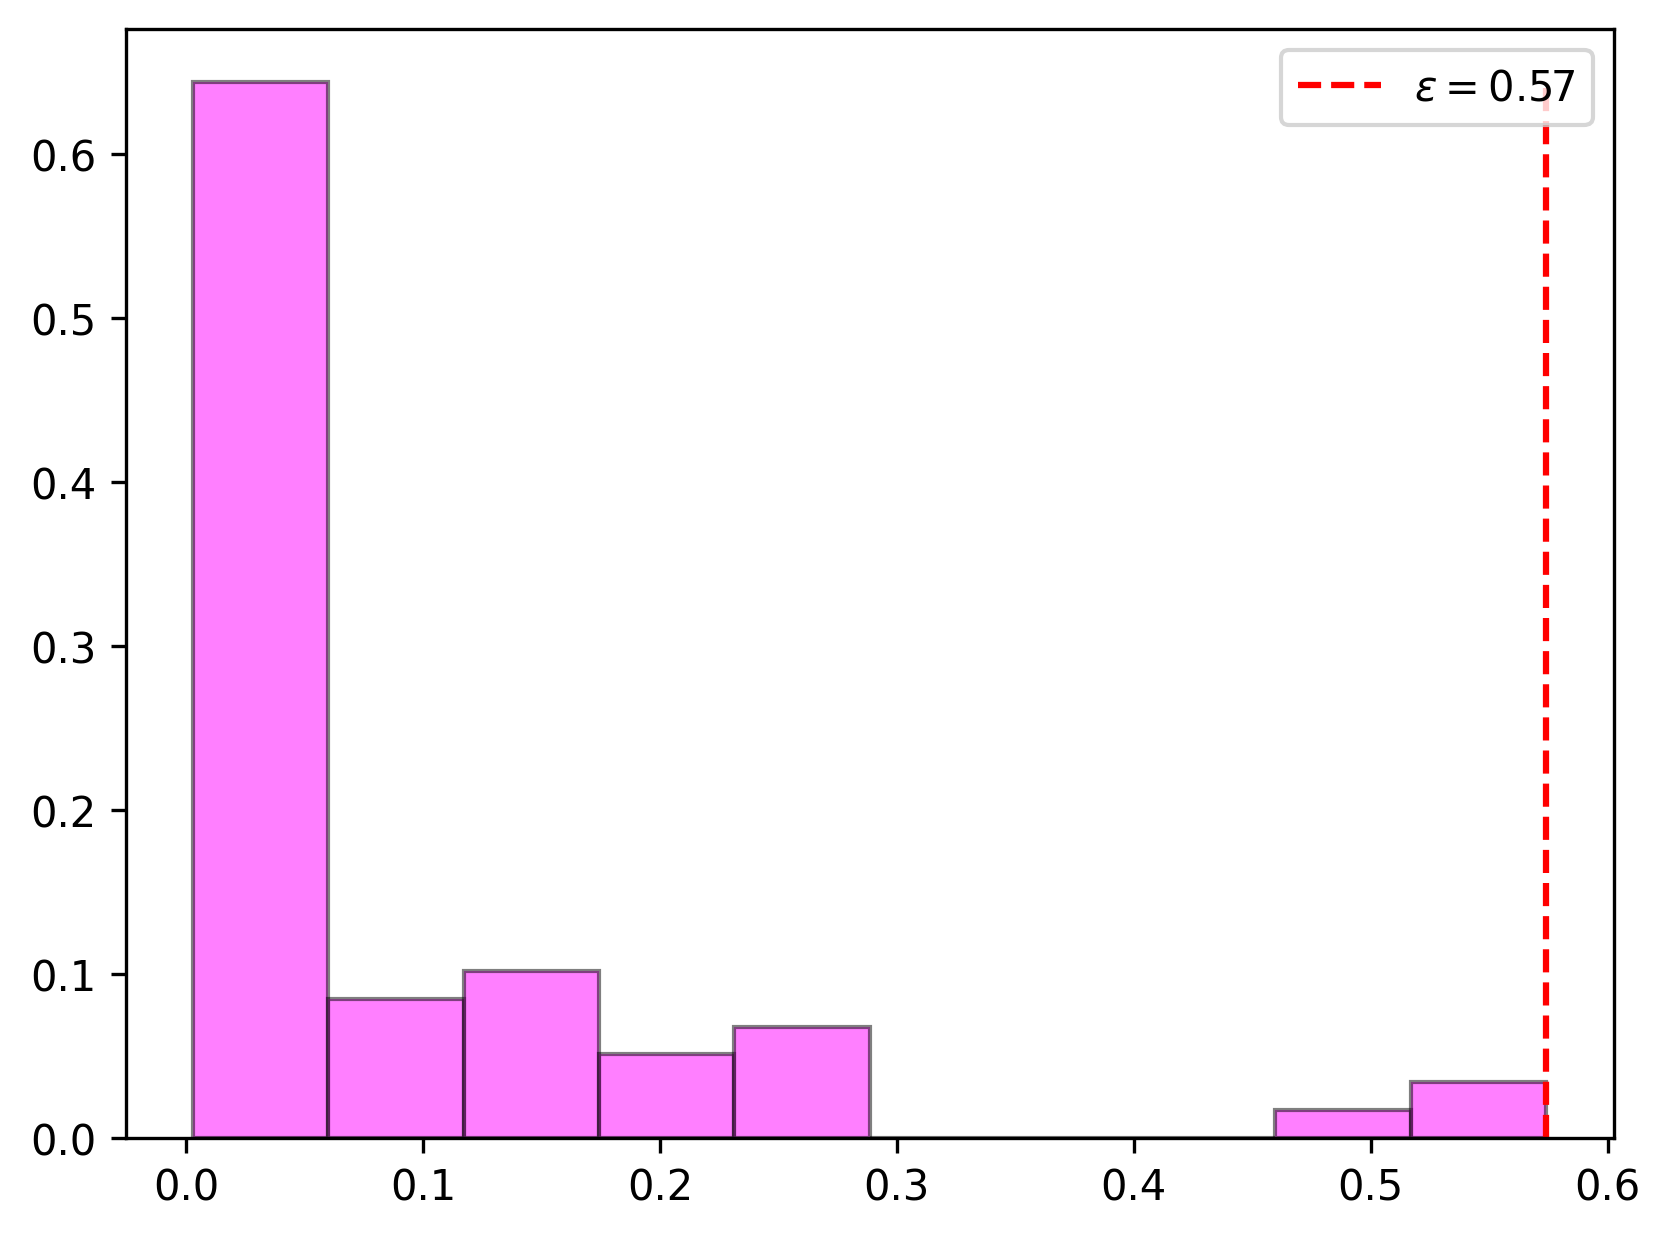
\includegraphics[width=\linewidth]{3-8-4}
			%\caption{fig}
		\end{minipage}
	}
	\subfigure[\scriptsize PnP-ADMM(IRCNN)]{
		\label{subfigure:3-1-3}
		\begin{minipage}[b]{0.18\linewidth}
			\centering
			\includegraphics[width=\linewidth]{3-8-5}\\
			\includegraphics[width=\linewidth]{3-8-6}
			%\caption{fig}
		\end{minipage}
	}
	\subfigure[\scriptsize TACE(IRCNN)]{
		\label{subfigure:3-1-4}
		\begin{minipage}[b]{0.18\linewidth}
			\centering
			\includegraphics[width=\linewidth]{3-8-7}\\
			\includegraphics[width=\linewidth]{3-8-8}
			%\caption{fig}
		\end{minipage}
	}
	\subfigure[\scriptsize PnP-FBS]{
		\label{subfigure:3-1-5}
		\begin{minipage}[b]{0.18\linewidth}
			\centering
			\includegraphics[width=\linewidth]{3-8-9}\\
			\includegraphics[width=\linewidth]{3-8-10}
			%\caption{fig}
		\end{minipage}
	}
	\caption{PnP-ADMM与TACE算法在迭代过程中的利普希茨常数分布直方图}
	\label{fig:3-8}
\end{figure}

图\ref{fig:3-8}中的\subref{subfigure:3-1-1}、\subref{subfigure:3-1-2}分别表示PnP-ADMM算法、TACE算法中数据保真项近邻算子与DnCNN去噪器在迭代过程中的利普希茨常数统计直方图;\subref{subfigure:3-1-3}、\subref{subfigure:3-1-4}分别表示PnP-ADMM算法、TACE算法中数据保真项近邻算子与IRCNN去噪器在迭代过程中的利普希茨常数统计直方图;\subref{subfigure:3-1-5}表示PnP-FBS在迭代过程中的利普希茨常数统计直方图,上层为DnCNN,下层为IRCNN;除\subref{subfigure:3-1-5}外上层代表数据保真项的近邻算子,下层代表图像去噪算子。从图\ref{fig:3-8}可以看出,在迭代过程中,盲DnCNN和IRCNN去噪算子满足利普希茨约束假设,而编码衍射模型的非凸数据保真项的近邻算子却不是非扩张算子,不满足假设\ref{assumption:3-2}。故该算法无法保证收敛到不动点,关于数据保真项的求解算法有待进一步研究。

\subsection{抗泊松噪声模型}
当式\eqref{equation:3-20}中的$\omega\sim{\mathcal{N}(0,\alpha\vert{Ax}\vert)}$时,观测值受泊松噪声的污染。表\ref{table:3-7}与表\ref{table:3-8}给出了不同噪声强度不同去噪算子下四种算法重构原始图像的PSNR/SSIM结果。
\begin{table}[!htbp]
	\def\arraystretch{1.4}\centering\zihao{5}
	\caption{不同算法在DnCNN下获得平均PSNR(dB)/SSIM比较}
	\label{table:3-7}
	\begin{tabular*}{\linewidth}{@{}@{\extracolsep{\fill}}cccccc@{}}
		\toprule
		算法 & prDeep & PnP-ADMM & PnP-FBS & TACE & 文献\cite{Kaixuan}\\ %\cmidrule(r){2-6}
		\midrule
		$\alpha=9$        & 37.35/0.9188   & 40.27/{\color{red}0.9638}  & {\color{red}40.33}/0.9635 & 40.20/0.9607 & {\color{red}40.33}/-  \\
		$\alpha=27$        & 32.53/0.8296   & 34.95/{\color{red}0.9210}  & {\color{red}35.02}/0.9096 & 34.95/0.9206  & 33.90/-	\\
		$\alpha=81$        & 28.51/0.8100   & 28.23/0.8052  & {\color{red}28.54}/{\color{red}0.8121} & 28.29/0.8073  & 27.23/-	\\
		\bottomrule
	\end{tabular*}
\end{table}
\begin{table}[!htbp]
	\def\arraystretch{1.4}\centering\zihao{5}
	\caption{不同算法在IRCNN下获得平均PSNR(dB)/SSIM比较}
	\label{table:3-8}
	\begin{tabular*}{\linewidth}{@{}@{\extracolsep{\fill}}ccccc@{}}
		\toprule
		算法     & prDeep & PnP-ADMM & PnP-FBS & TACE\\ %\cmidrule(r){2-5}
		\midrule
		$\alpha=9$         & 37.34/0.9188   & 39.63/{\color{red}0.9619}  & {\color{red}39.78}/0.9613 & 39.55/0.9587\\
		$\alpha=27$        & 32.43/0.8325   & 34.64/0.9209  & {\color{red}34.83}/{\color{red}0.9220} & 34.63/0.9200\\
		$\alpha=81$        & 28.45/0.8214   & 28.32/0.8230  & {\color{red}28.49}/{\color{red}0.8245} & 28.23/0.8220\\
		\bottomrule
	\end{tabular*}
\end{table}

从表\ref{table:3-7}与表\ref{table:3-8}可以看出,TACE算法的重构图像质量高于peDeep算法,并且与PnP-ADMM算法结果接近,验证了PnP-ADMM与TACE收敛到相同的不动点。由于PnP-FBS使用了自适应迭代步长技术,使得该算法为SOTA结果。但是TACE算法在不同尺度泊松噪声下,对比文献\cite{Kaixuan}提出的基于强化学习的深度展开即插即用算法,PSNR的差值按泊松噪声污染强度由小到大依次为-0.13dB、1.05dB、1.06dB(TACE算法减去文献\cite{Kaixuan}所提的算法)。需要注意的是二者的观测矩阵不同。但通过二者较大的数值差距,可以看出TACE算法在泊松噪声强度较大的情况下优于文献\cite{Kaixuan}所提的算法。

为衡量算法的计算复杂度,本小节给出了算法的平均运行时间。表\ref{table:3-9}给出了四种算法在不同去噪算子下的GPU运行时间,关于平均运行时间的结论与上节高斯噪声的相同。
\begin{table}[!htbp]
	\def\arraystretch{1.4}\centering\zihao{5}
	\caption{不同算法不同去噪器在Barbara上的运行时间(s)($\alpha=81$)}
	\label{table:3-9}
	\begin{tabular*}{\linewidth}{@{}@{\extracolsep{\fill}}ccccc@{}}
		\toprule
		算法 & prDeep & PnP-ADMM & PnP-FBS & TACE	\\ %\cmidrule(r){2-5}
		\midrule
		512 x 512        & {\color{blue}27.78}/{\color{blue}9.15}   & 28.41/9.79  & 28.43/9.47 & 30.83/11.26\\
		Device	         & GPU   & GPU  & GPU 	& GPU \\
		\bottomrule
	\end{tabular*}
\end{table}

图\ref{fig:3-9}与图\ref{fig:3-10}给出了不同算法在DnCNN和IRCNN去噪算子下$\alpha=81$时Barbara与Pollen的重构结果,主观视觉结论与上节相同。
\begin{figure}[!htbp]
	\centering
	\subfigure[\scriptsize Original]{
		\includegraphics[width=0.18\linewidth]{3-9-1}
	}\hspace{-0.01\linewidth}
	\subfigure[\scriptsize prDeep/27.25]{
		\includegraphics[width=0.18\linewidth]{3-9-2}
	}\hspace{-0.01\linewidth}
	\subfigure[\scriptsize PnP-ADMM/26.80]{
		\includegraphics[width=0.18\linewidth]{3-9-3}
	}\hspace{-0.01\linewidth}
	\subfigure[\scriptsize PnP-FBS/{\color{red}27.26}]{
		\includegraphics[width=0.18\linewidth]{3-9-4}
	}\hspace{-0.01\linewidth}
	\subfigure[\scriptsize TACE/26.89]{
		\includegraphics[width=0.18\linewidth]{3-9-5}
	}

	\subfigure[\scriptsize Original]{
		\includegraphics[width=0.18\linewidth]{3-9-6}
	}\hspace{-0.01\linewidth}
	\subfigure[\scriptsize prDeep/25.80]{
		\includegraphics[width=0.18\linewidth]{3-9-7}
	}\hspace{-0.01\linewidth}
	\subfigure[\scriptsize PnP-ADMM/25.45]{
		\includegraphics[width=0.18\linewidth]{3-9-8}
	}\hspace{-0.01\linewidth}
	\subfigure[\scriptsize PnP-FBS/{\color{red}25.82}]{
		\includegraphics[width=0.18\linewidth]{3-9-9}
	}\hspace{-0.01\linewidth}
	\subfigure[\scriptsize TACE/25.55]{
		\includegraphics[width=0.18\linewidth]{3-9-10}
	}
	\caption{Barbara与Pollen重构结果($\alpha=81$,DnCNN)} 
	\label{fig:3-9}
\end{figure}
\begin{figure}[!htbp]
	\setlength{\belowcaptionskip}{-0.01\linewidth}
	\centering
	\subfigure[\scriptsize Original]{
		\includegraphics[width=0.18\linewidth]{3-10-1}
	}\hspace{-0.01\linewidth}
	\subfigure[\scriptsize prDeep/26.86]{
		\includegraphics[width=0.18\linewidth]{3-10-2}
	}\hspace{-0.01\linewidth}
	\subfigure[\scriptsize PnP-ADMM/26.54]{
		\includegraphics[width=0.18\linewidth]{3-10-3}
	}\hspace{-0.01\linewidth}
	\subfigure[\scriptsize PnP-FBS/{\color{red}26.88}]{
		\includegraphics[width=0.18\linewidth]{3-10-4}
	}\hspace{-0.01\linewidth}
	\subfigure[\scriptsize TACE/26.57]{
		\includegraphics[width=0.18\linewidth]{3-10-5}
	}

	\subfigure[\scriptsize Original]{
		\includegraphics[width=0.18\linewidth]{3-10-6}
	}\hspace{-0.01\linewidth}
	\subfigure[\scriptsize prDeep/25.80]{
		\includegraphics[width=0.18\linewidth]{3-10-7}
	}\hspace{-0.01\linewidth}
	\subfigure[\scriptsize PnP-ADMM/25.53]{
		\includegraphics[width=0.18\linewidth]{3-10-8}
	}\hspace{-0.01\linewidth}
	\subfigure[\scriptsize PnP-FBS/{\color{red}25.81}]{
		\includegraphics[width=0.18\linewidth]{3-10-9}
	}\hspace{-0.01\linewidth}
	\subfigure[\scriptsize TACE/25.61]{
		\includegraphics[width=0.18\linewidth]{3-10-10}
	}
	\caption{Barbara与Pollen重构结果($\alpha=81$,IRCNN)} 
	\label{fig:3-10}
\end{figure}

图\ref{fig:3-11}给出了PnP-ADMM与TACE算法中各个代理在迭代过程中的利普希茨常数统计直方图,测试图像为Barbara,$\alpha=81$。图\ref{fig:3-11}中的\subref{subfigure:3-2-1}、\subref{subfigure:3-2-2}分别表示PnP-ADMM算法、TACE算法中数据保真项近邻算子与DnCNN去噪器在迭代过程中的利普希茨常数统计直方图;\subref{subfigure:3-2-3}、\subref{subfigure:3-2-4}表示PnP-ADMM算法、TACE算法中数据保真项近邻算子与IRCNN去噪器在迭代过程中的利普希茨常数统计直方图;\subref{subfigure:3-2-5}表示PnP-FBS在迭代过程中的利普希茨常数统计直方图,上层为DnCNN,下层为IRCNN;除\subref{subfigure:3-2-5}外上层代表数据保真项的近邻算子,下层代表图像去噪算子。关于TACE算法两个代理利普希茨常数的结论与上节高斯噪声的结论相同。
\begin{figure}[!htbp]
	\centering
	\subfigure[\scriptsize PnP-ADMM(DnCNN)]{
		\label{subfigure:3-2-1}
		\begin{minipage}[b]{0.18\linewidth}
			\centering
			\includegraphics[width=\linewidth]{3-11-1}\\
			\includegraphics[width=\linewidth]{3-11-2}
			%\caption{fig}
		\end{minipage}
	}
	\subfigure[\scriptsize TACE(DnCNN)]{
		\label{subfigure:3-2-2}
		\begin{minipage}[b]{0.18\linewidth}
			\centering
			\includegraphics[width=\linewidth]{3-11-3}\\
			\includegraphics[width=\linewidth]{3-11-4}
			%\caption{fig}
		\end{minipage}
	}
	\subfigure[\scriptsize PnP-ADMM(IRCNN)]{
		\label{subfigure:3-2-3}
		\begin{minipage}[b]{0.18\linewidth}
			\centering
			\includegraphics[width=\linewidth]{3-11-5}\\
			\includegraphics[width=\linewidth]{3-11-6}
			%\caption{fig}
		\end{minipage}
	}
	\subfigure[\scriptsize TACE(IRCNN)]{
		\label{subfigure:3-2-4}
		\begin{minipage}[b]{0.18\linewidth}
			\centering
			\includegraphics[width=\linewidth]{3-11-7}\\
			\includegraphics[width=\linewidth]{3-11-8}
			%\caption{fig}
		\end{minipage}
	}
	\subfigure[\scriptsize PnP-FBS]{
		\label{subfigure:3-2-5}
		\begin{minipage}[b]{0.18\linewidth}
			\centering
			\includegraphics[width=\linewidth]{3-11-9}\\
			\includegraphics[width=\linewidth]{3-11-10}
			%\caption{fig}
		\end{minipage}
	}
	\caption{PnP-ADMM与TACE算法在迭代过程中的利普希茨常数分布直方图}
	\label{fig:3-11}
\end{figure}

\section{本章小结}
本章首先介绍了基于即插即用先验的PnP-ADMM和PnP-FBS算法与基于RED先验的prDeep算法,其次推导了共识优化到共识方程的推演过程,最后提出了基于共识方程的编码衍射成像算法,并在数据保真项近邻算子和去噪算子非扩张的假设下,该算法收敛到全局的不动点。实验结果证明了在重构实图像时,该算法的重构性能与即插即用ADMM算法相当,且略低于即插即用邻近梯度算法;其次,通过数据保真项近邻算子和去噪算子在迭代过程中的利普希茨常数统计直方图验证了该算法的收敛性。
%本章提出了针对非凸反问题的具有收敛性保证的可学习迭代方法框架,并提供了显式动量和隐式动量两种情况下的收敛性分析。该框架具有极高的灵活性,可以把大部分现有的可学习优化方法囊括进来并进行带有收敛性分析的改进。同时,该框架的理论结果也解释了可学习的深度网络能够学习到某一指定函数的下降方向,为网络的可解释性提供了一些可能性。在视觉问题上的实验也验证了本文方法的有效性。

